\documentclass{beamer}
\usetheme{}
\usecolortheme{dolphin}           
\useinnertheme{circles}
\setbeamertemplate{itemize items}[default]
\setbeamertemplate{enumerate items}[default]
\usepackage[T1]{fontenc}
\usepackage[utf8]{inputenc}
\usepackage{lmodern}
\usepackage{amsmath}
\usepackage{booktabs} 
\usepackage{graphicx}        
\usepackage{array}
\usepackage{color}
\makeatletter
\def\zapcolorreset{\let\reset@color\relax\ignorespaces}
\def\colorrows#1{\noalign{\aftergroup\zapcolorreset#1}\ignorespaces}
\makeatother
\graphicspath{{/home/swl/Dropbox/ucd/advanced_macro/figures/}} 
\setbeamertemplate{navigation symbols}{}

%--------------------------------------
\title{Growth accounting}
\author{School of Economics, University College Dublin}
\date{Spring 2018}
\begin{document}

%--------------------------------------
\begin{frame}
 \titlepage
\end{frame}
%--------------------------------------

%--------------------------------------
\begin{frame}
  \begin{figure}
    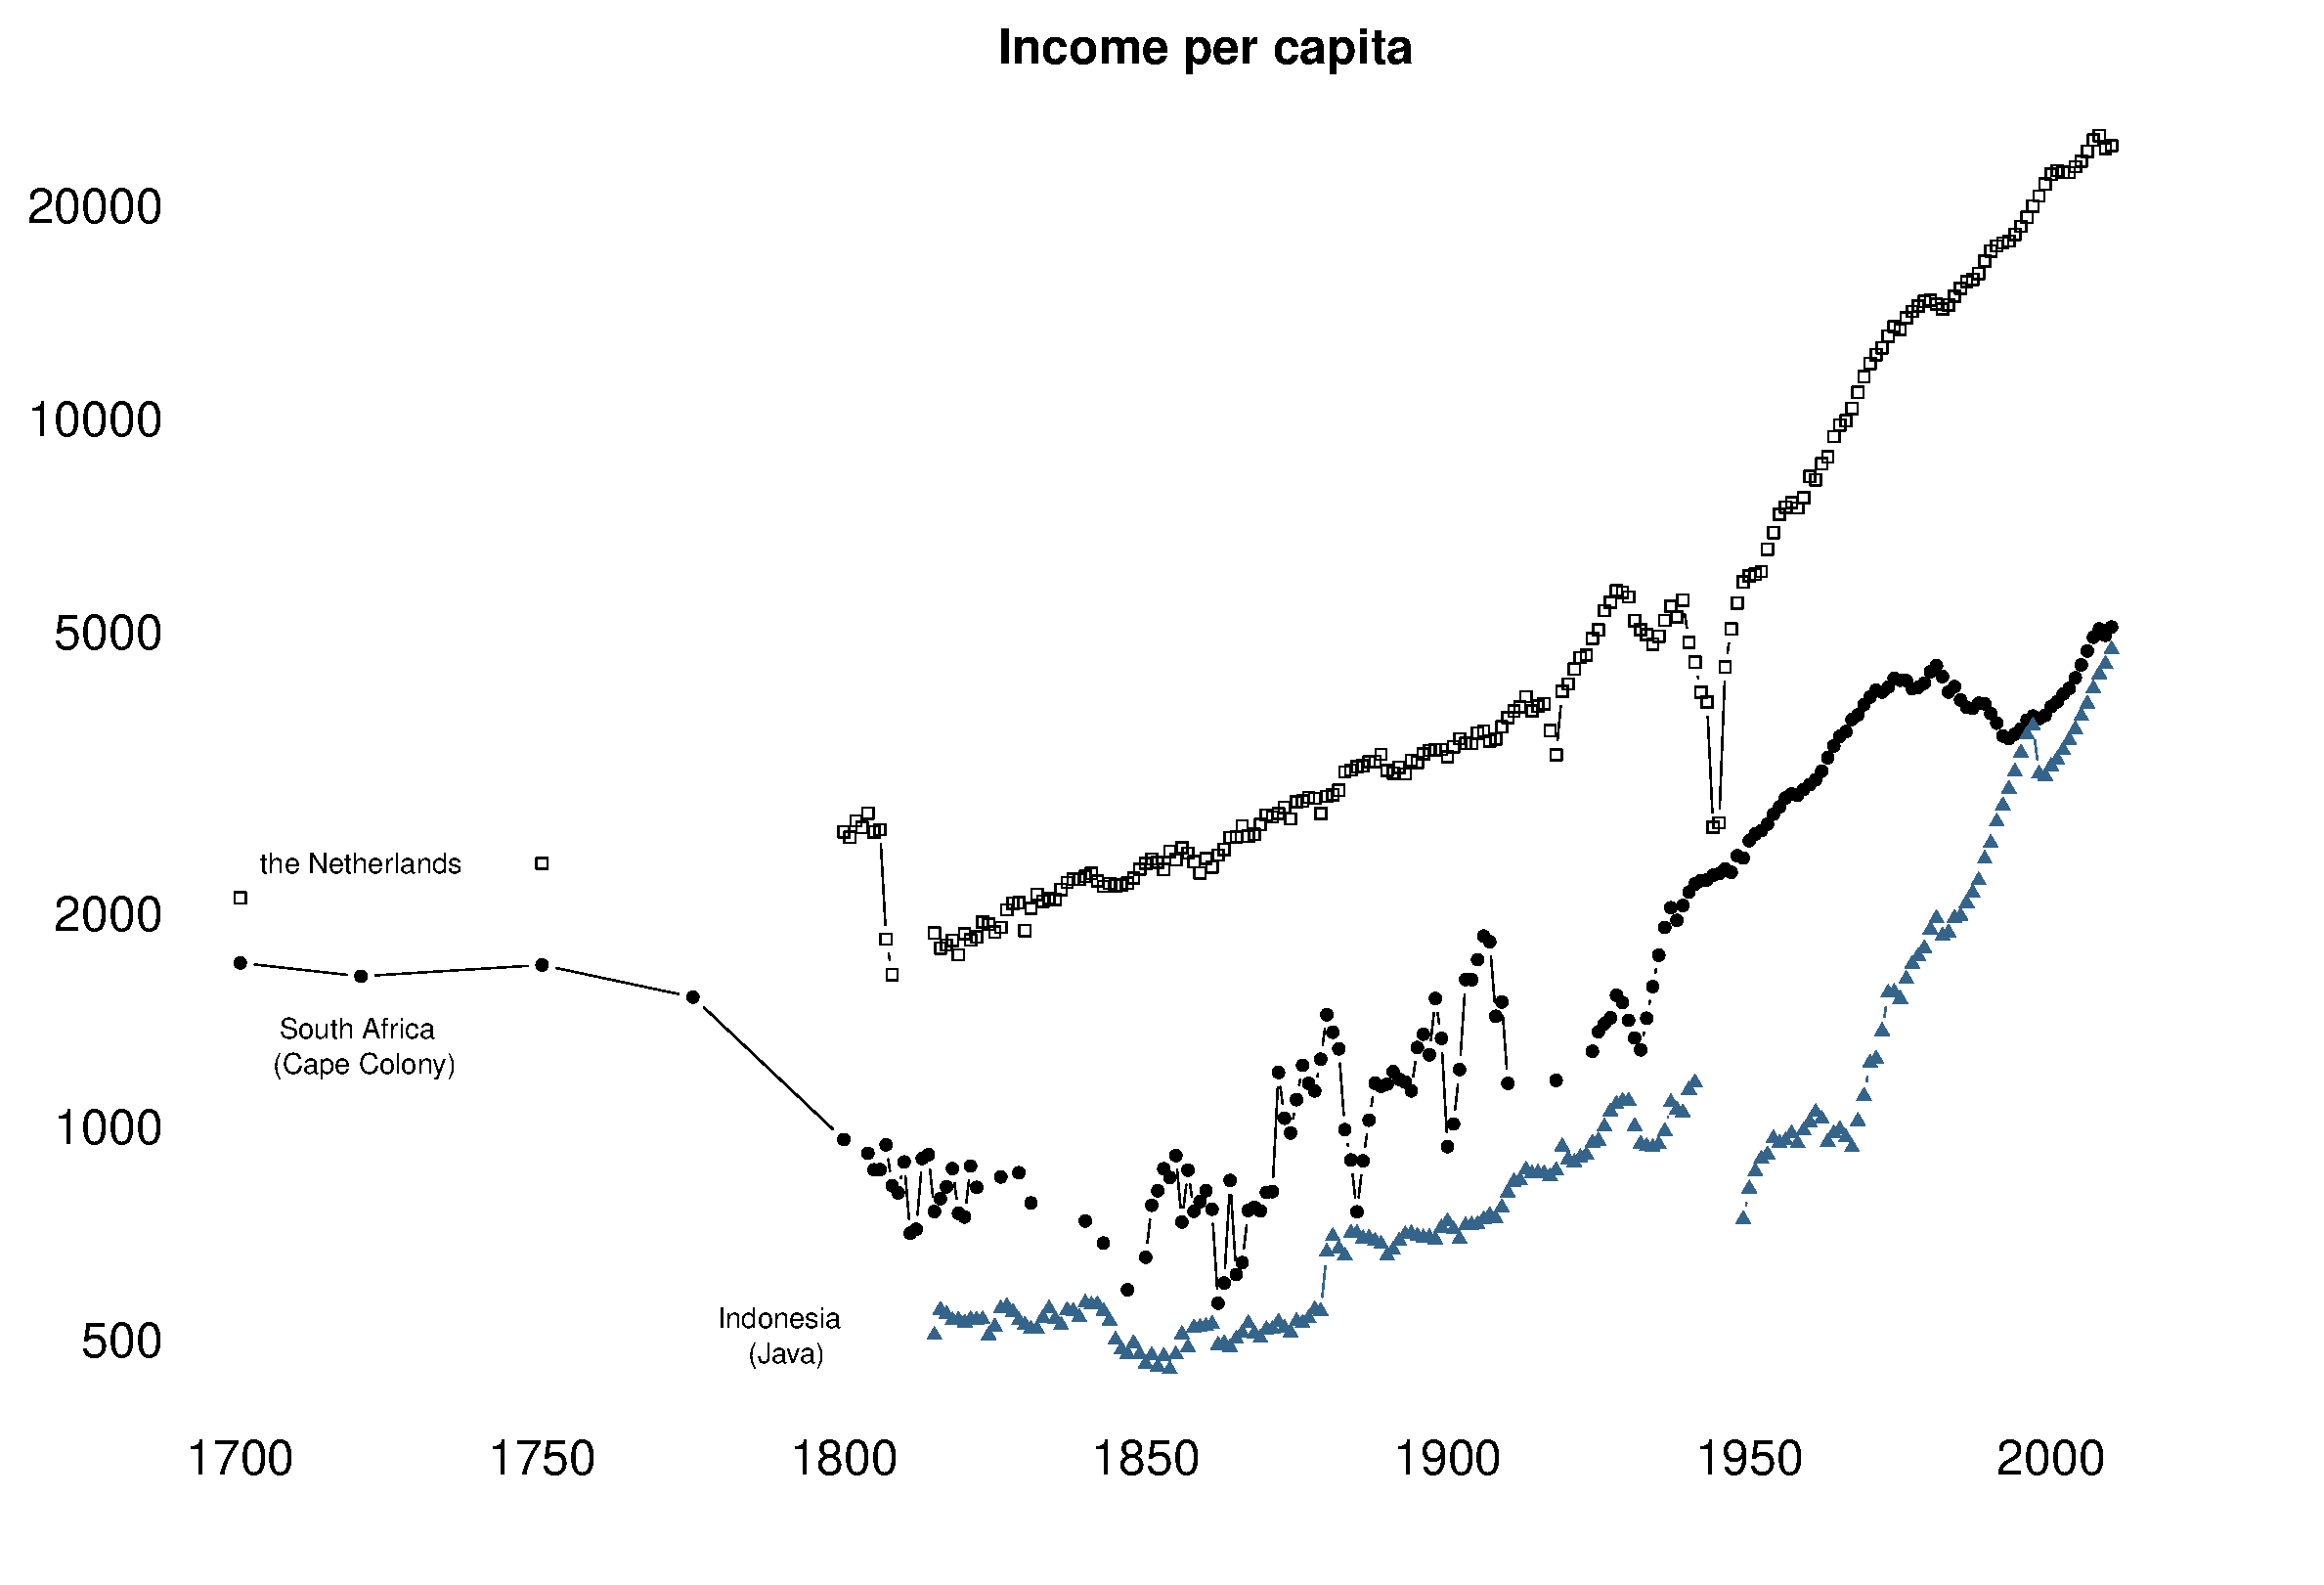
\includegraphics[scale=.3]{historic_income.eps}
  \end{figure}
\end{frame}
%--------------------------------------

%--------------------------------------
\begin{frame}
  A stylised fact from economic history: standards of living have been roughly similar in Assyria (1500 BCE), Roman Egypt, and late 18th century England (Clark, 2007)
  \begin{itemize}
    \item Strong link between income per capita and income growth
    \item Any increases in aggregate outcome offset by increase in population size
  \end{itemize}
  \medskip
  In this Malthusian world income per capita remains at constant level, despite technological progress
  \begin{enumerate}
    \item Long-run stagnation
    \item Population growth will outpace agricultural productivity
  \end{enumerate}
\end{frame}
%--------------------------------------

%--------------------------------------
\begin{frame}
  Empirical predictions of the Malthusian model are not that impressive
  \begin{itemize}
    \item Specifically that mortality should rise as living standards fall (Kelly \& O'Grada, 2014)
  \end{itemize}
  \medskip
  Nonetheless, the Malthusian has had great influence on economic thinking
  \begin{itemize}
    \item Research on environment and conflict
    \item 'Shithole countries' 
  \end{itemize}
\end{frame}
%--------------------------------------

%--------------------------------------
\begin{frame}
  \begin{figure}
    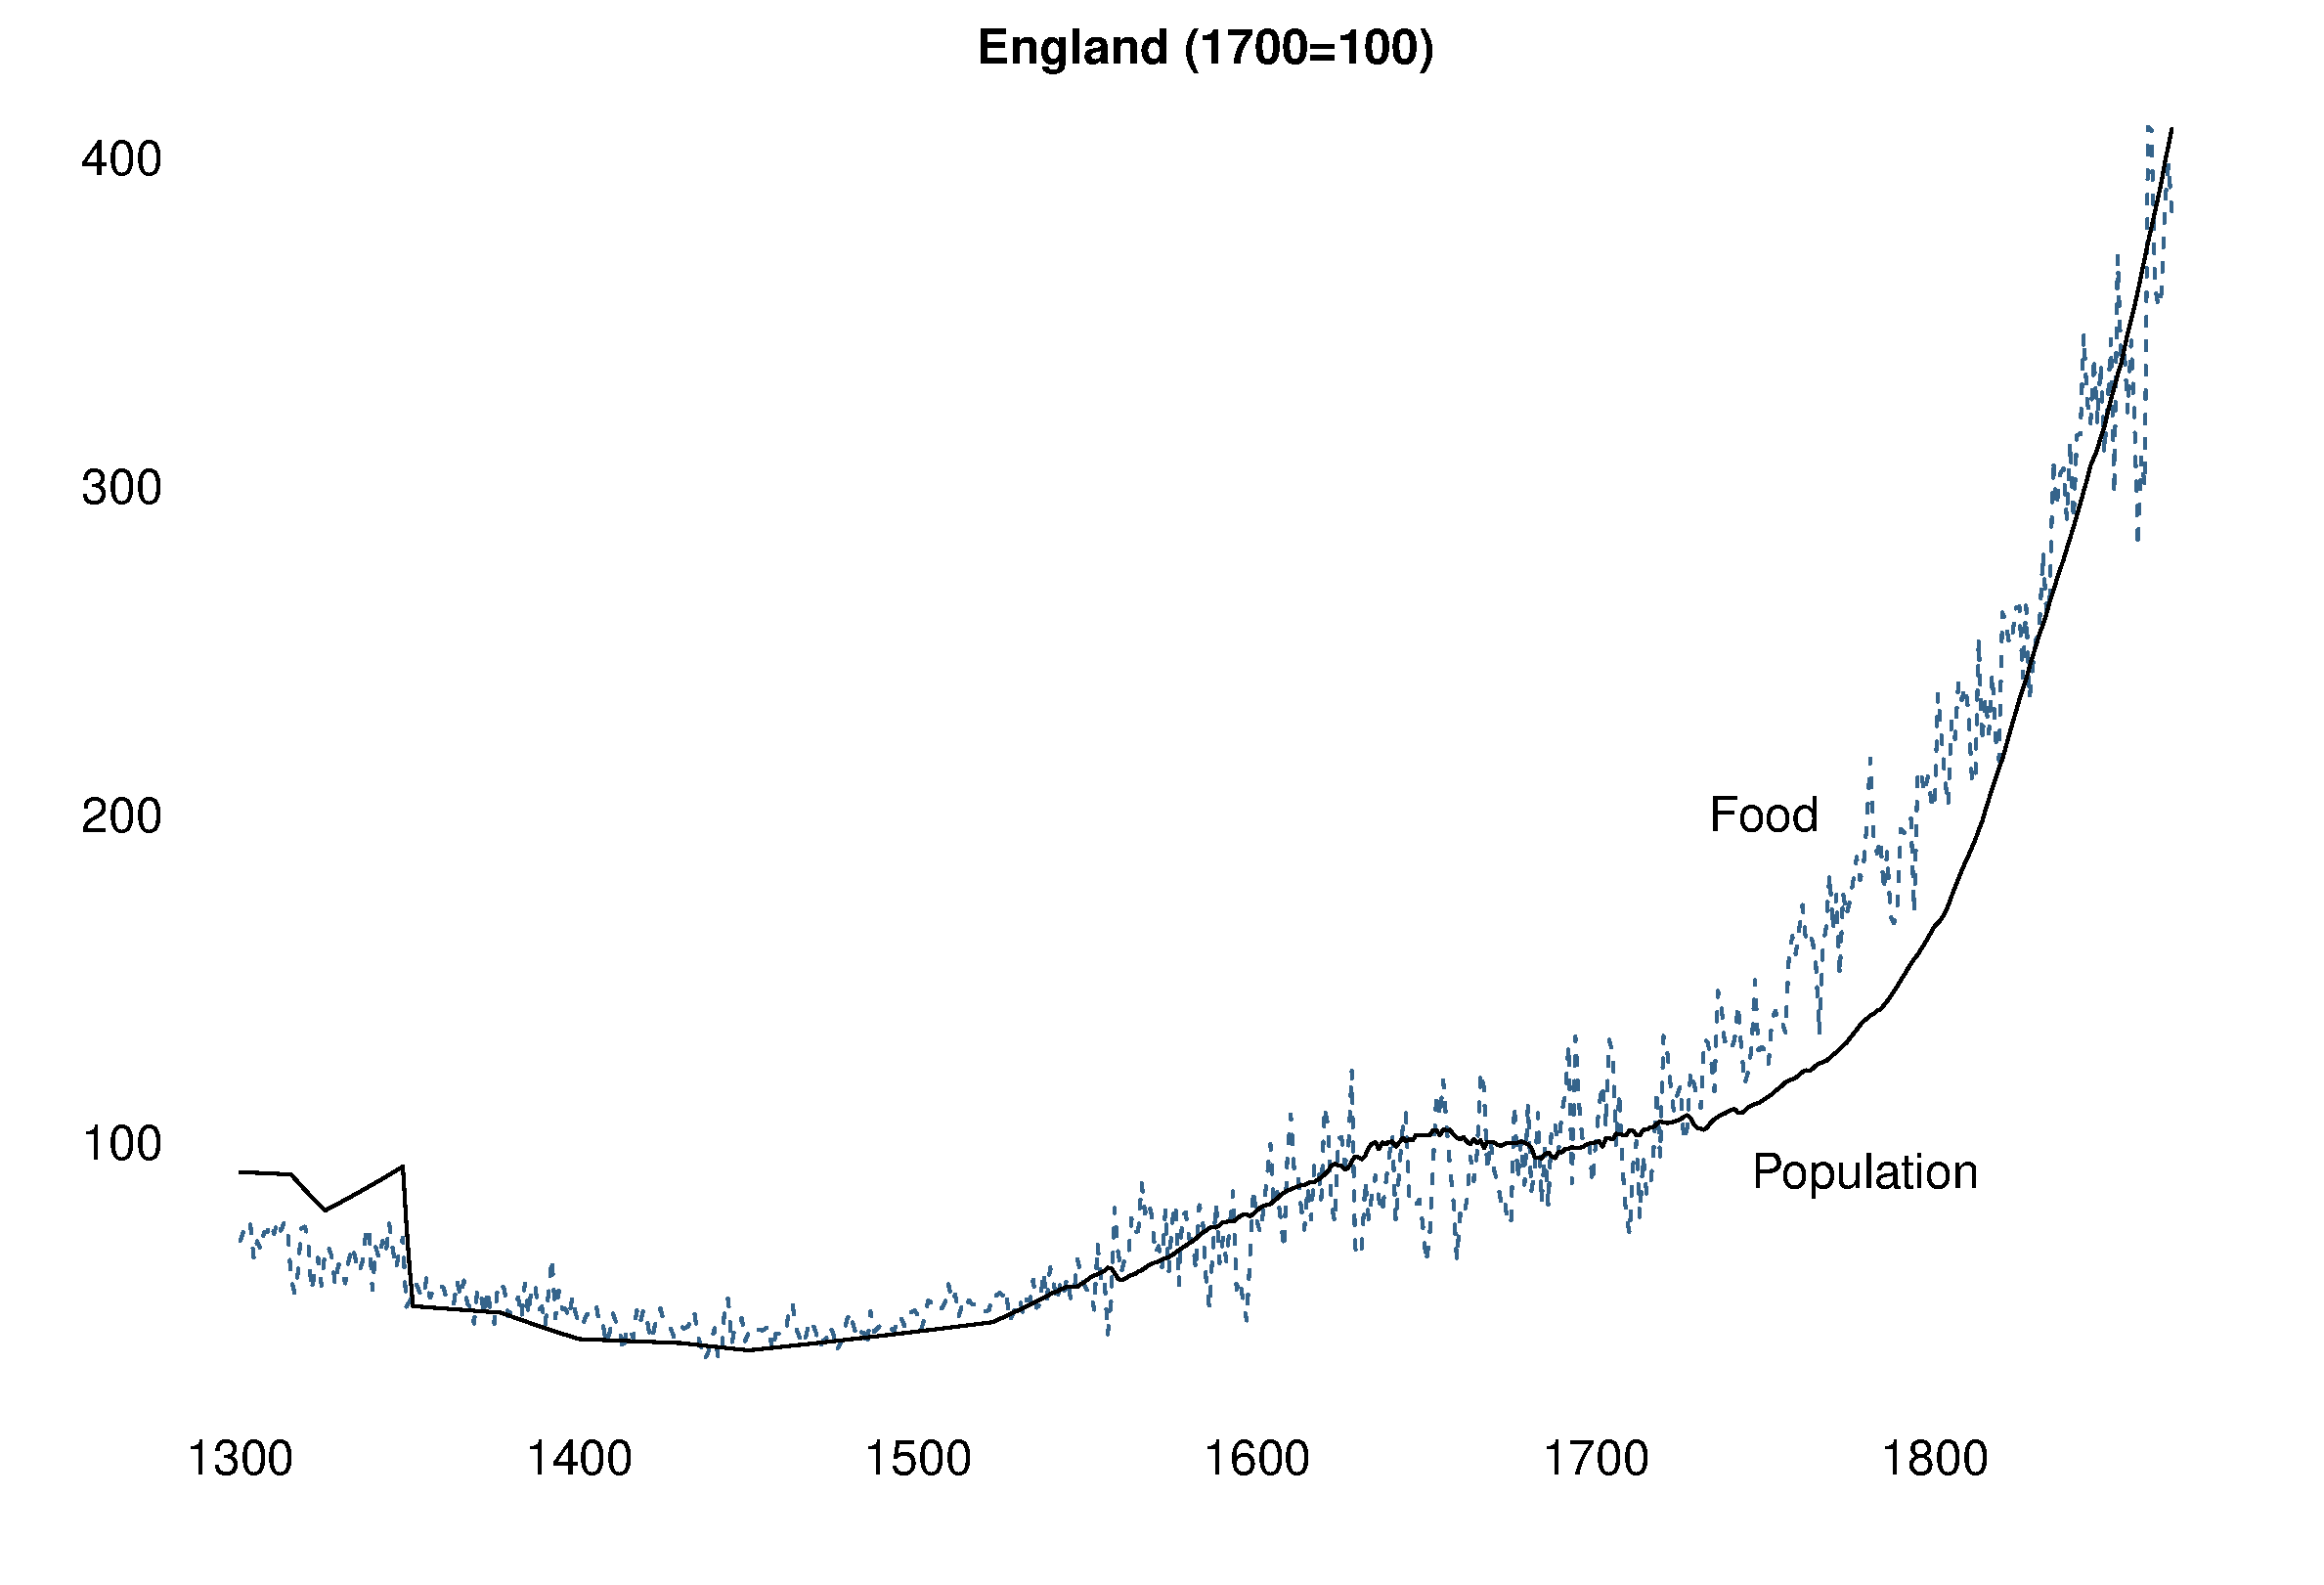
\includegraphics[scale=.3]{malthus.eps}
  \end{figure}  
\end{frame}
%--------------------------------------

%--------------------------------------
\begin{frame}
  \begin{figure}
    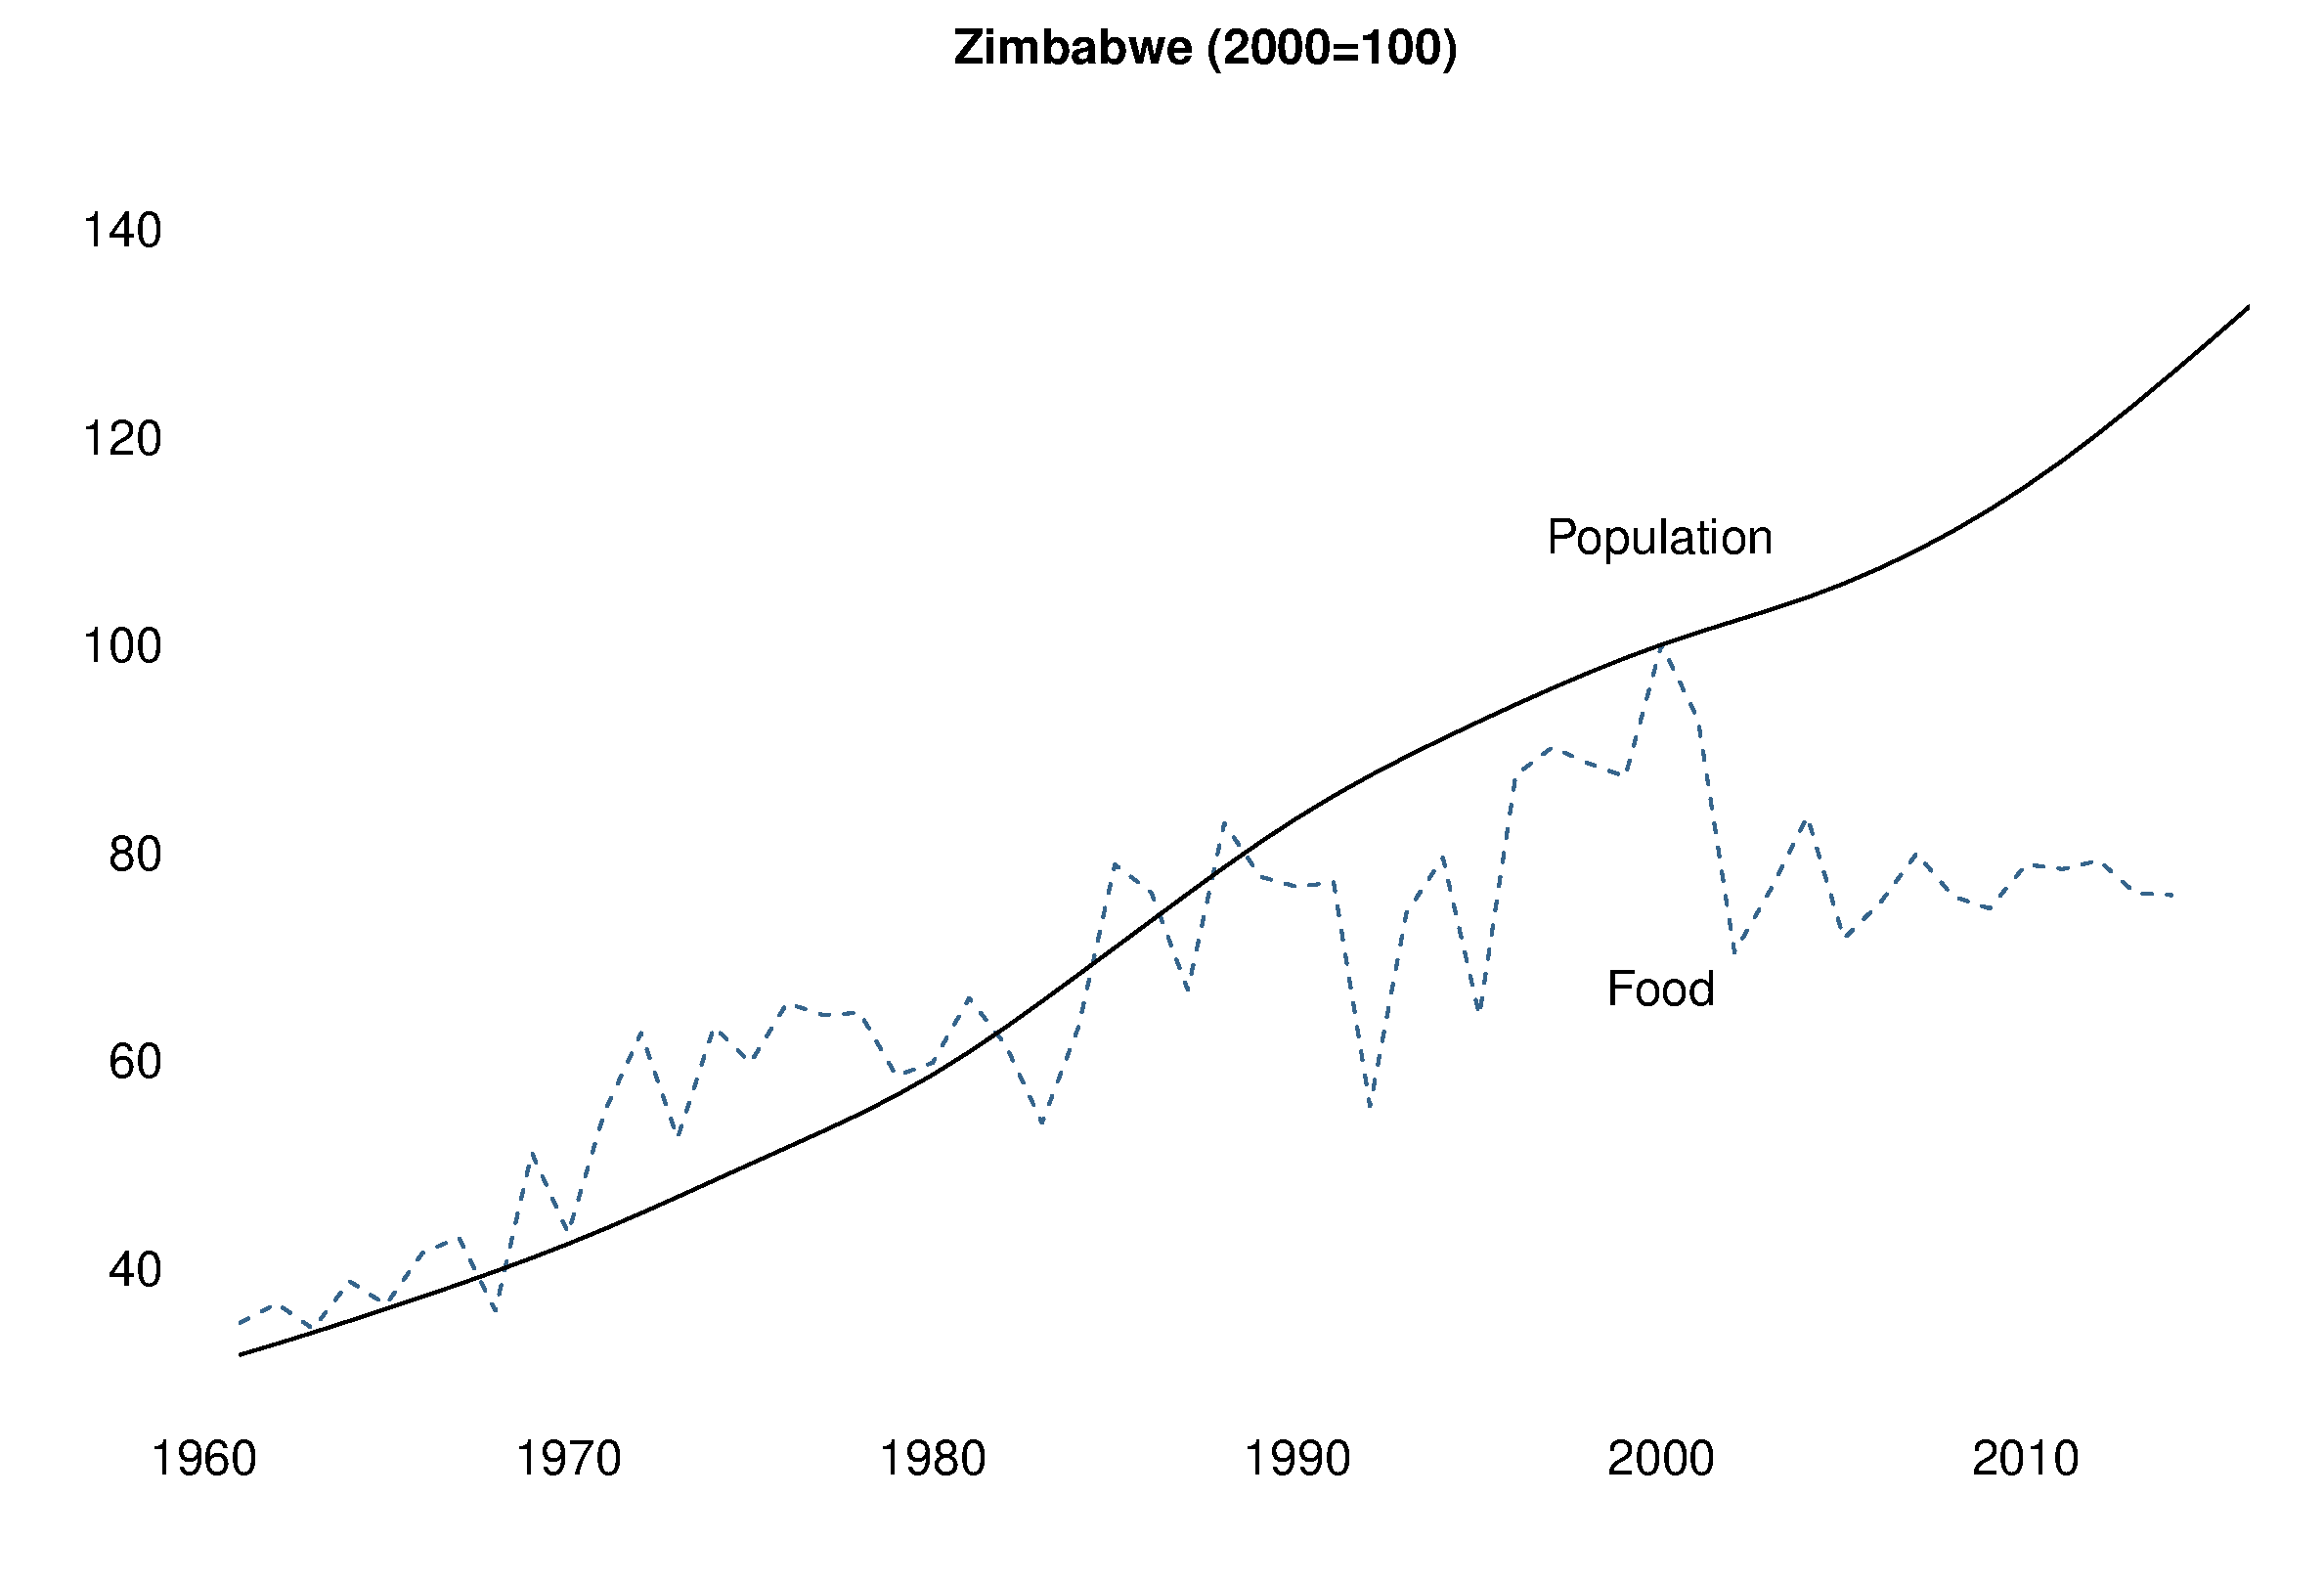
\includegraphics[scale=.3]{malthus2.eps}
  \end{figure}  
\end{frame}
%--------------------------------------

%--------------------------------------
\begin{frame}
 Let's consider a Malthusian model where output is determined by two factors 
 \begin{enumerate}
   \item Land $X$
   \item Labour $L$
 \end{enumerate}
 \medskip
 For simplicity we assume that
 \begin{itemize}
   \item Amount of land is fixed
   \item Labour force = total population
 \end{itemize} 
\end{frame}
%--------------------------------------

%--------------------------------------
\begin{frame}
  Aggregate production function can be written as  
  \begin{align}
    Y=AX^{\alpha}L^{1-\alpha}
  \end{align}
  \medskip
  $Y$ is total aggregate output\\
  $A$ is technology parameter\\
  $\alpha$ is output elasticity
\end{frame}
%--------------------------------------

%--------------------------------------
\begin{frame}
  Output $Y$ will increase when total population $L$ increases
  \begin{align}
    \frac{\partial Y}{\partial L} &= (1-\alpha)AX^{\alpha}L^{-\alpha}\\
  &= (1-\alpha)A \left( \frac{X}{L} \right)^{\alpha} > 0
  \end{align}  
\end{frame}
%--------------------------------------

%--------------------------------------
\begin{frame}
  The marginal product is positive but it will decrease given that $L$ is in the denominator  
  \begin{align}
    \frac{\delta^2Y}{\delta L^2} = -\alpha(1-\alpha)AX^{\alpha}L^{-\alpha-1}<0
  \end{align}
\end{frame}
%--------------------------------------

%--------------------------------------
\begin{frame}
  To measure living standards we can use output per capita $y$.\\  
  Take 
  \begin{align}
    Y=AX^{\alpha}L^{1-\alpha}
  \end{align}
  and divide by $L$
  \begin{align}
    \frac{Y}{L} &= \frac{AX^{\alpha}L^{1-\alpha}}{L}\\
    &= A\left ( \frac{X}{L} \right)^{\alpha} = Ax^{\alpha} = y
  \end{align}
  $x$ is land per capita
\end{frame}
%--------------------------------------

%--------------------------------------
\begin{frame}
  Increase in population size will have two effects on living standards  
  \begin{enumerate}
    \item Production increase, resulting in increase in living standards
    \item More people to share production with, meaning a decrease in living standards
  \end{enumerate}
  \medskip
  In the Malthusian framework effect 2 will dominate, therefore population growth will lead to a fall in living standards.  
\end{frame}
%--------------------------------------

%--------------------------------------
\begin{frame}
 More formally;
 \begin{align}
  \frac{\partial y}{\partial L} &= -\alpha AX^{\alpha}L^{-\alpha-1} <0\\
  \frac{\partial^2 y}{\partial L^2} &= \alpha(1-\alpha)AX^{\alpha}L^{-\alpha-2}>0
 \end{align}  
\end{frame}
%--------------------------------------

%--------------------------------------
\begin{frame}
 Let's have a closer look at the population dynamics: In the model population size $L_t$ equals last year's population size plus the number of births $B_t$ and minus the number of deaths $D_t$ during the same year
  \begin{align}
   L_t = L_{t-1} + B_t(y_{t-1}) - D_t(y_{t-1})
  \end{align}
  \medskip
  Key feature here is that the number of births and deaths is a function of living standards or output per capita, lagged one year: $y_{t-1}$
  \begin{align}
    B'(y_{t-1})&>0\\
    D'(y_{t-1})&<0  
  \end{align}
  \medskip
  For simplicity the birth and death rate are assumed to be linear functions of output.
\end{frame}
%--------------------------------------

%--------------------------------------
\begin{frame} 
  \begin{figure}
    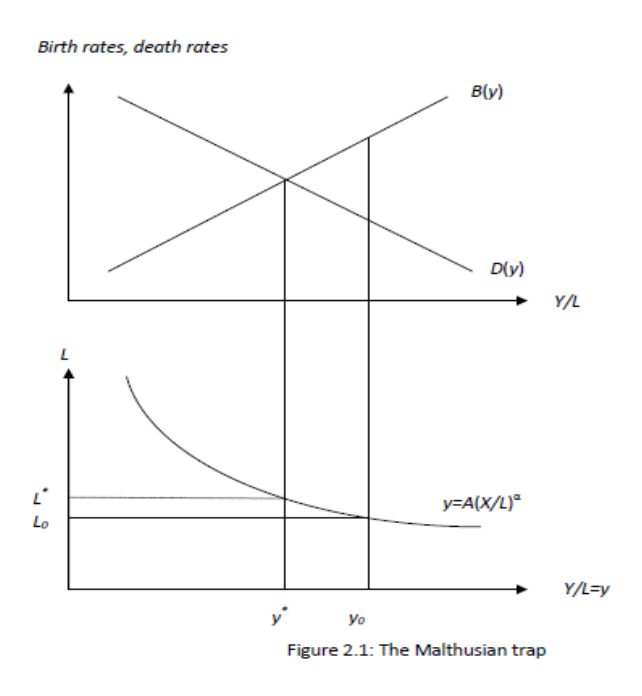
\includegraphics[scale=.7]{malthusian_trap.eps}
  \end{figure}
\end{frame}
%--------------------------------------

%--------------------------------------
\begin{frame}
  When output per capita increases, the food supply will increase which allows families to expand and reduce mortality due to better nourishment. 
  Output per capita will tend to converge towards an equilibrium indicated by $y^*$, at which point the population ceases to grow.
  \begin{itemize}
    \item This is known as the subsistence level
  \end{itemize}
  \begin{align}
  L_t-L_{t-1} = B_t(y^*)-D_t(y^*)=0
  \end{align}
\end{frame}
%--------------------------------------

%--------------------------------------
\begin{frame}
  Consider the case where we start at a relatively high output level, $y^0$.
  Given the relatively high output per capita there will be (relatively)
  \begin{itemize}
    \item Few deaths
    \item Many births
  \end{itemize}
  \medskip
  This will increase the population, decreasing living standards shifting the equilibrium to the left. 
  \begin{itemize}
    \item One can imagine a scenario starting at the left of the equilibrium where many people die and few children are born
    \item In this case the shrinking population will increase output per capita
  \end{itemize}
\end{frame}
%--------------------------------------

%--------------------------------------
\begin{frame}
  \begin{figure}
    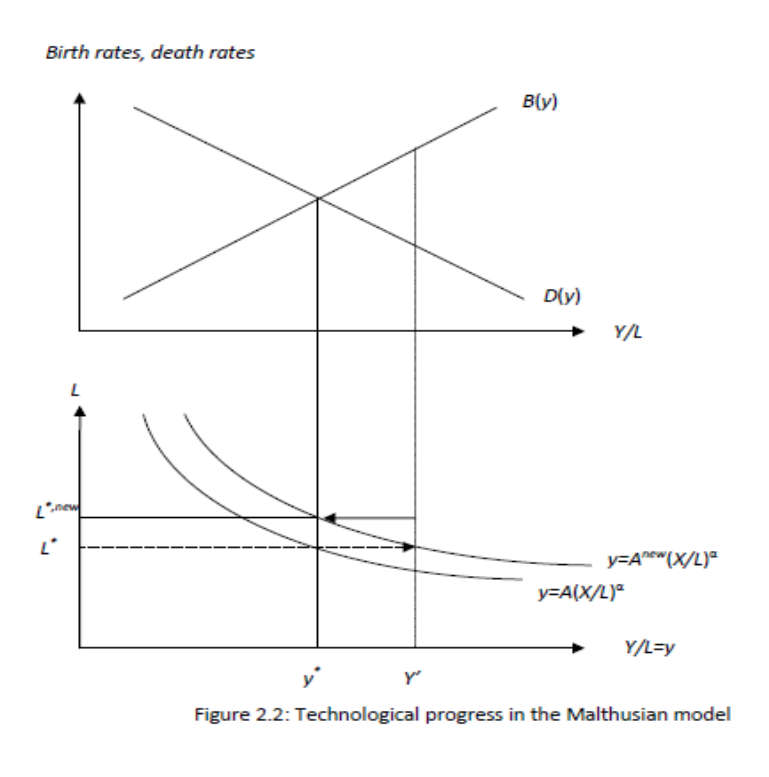
\includegraphics[scale=.7]{tech_progress.eps}
  \end{figure}
\end{frame}
%--------------------------------------

%--------------------------------------
\begin{frame}
  Following a positive technology shocks there will be an increase in productivity:   
  Productivity increase will shift equilibrium punt outward on $y$-curve: temporary increase in output per capita
  \begin{itemize}    
    \item This will increase birth rate and decrease death rate
    \item Population will increase reducing the living standards
  \end{itemize}
  \medskip
  As such, the only lasting thing of a technology shock is a larger population.
\end{frame}
%--------------------------------------

%--------------------------------------
\begin{frame}
 History has shown that there are a number of factors contributing to a break with the Malthusian trap:
\begin{enumerate}
  \item Fall in birth rate ending link with income per capita
  \item Increase in education level
  \item Increase in growth of technological knowledge
  \item Increase in output per capita far beyond subsistence level
\end{enumerate}
\end{frame}
%--------------------------------------

%--------------------------------------
\begin{frame}
 Moving on to the Cobb-Douglas model  
\begin{align}
  Y_t=A_tK^{\alpha}_tL^{\beta}_t
\end{align}
  \medskip
  Assume that output is determined by an aggregate production function technology depending on the total amount of labour ($L$) and capital ($K$). 
\end{frame}
%--------------------------------------

%--------------------------------------
\begin{frame}
  In the Cobb-Douglas model $A_t$ accounts for technology, a measure for productive efficiency
\begin{itemize}
  \item Increase in $A_t$ results in higher output without having to raise inputs
  \item Fluctuates for various reasons, e.g. new technology, government regulation, better management
\end{itemize} 
\medskip
Since $A_t$ increases productiveness of other factors, it is also known as Total Factor Productivity (TFP)
\end{frame}
%--------------------------------------

%--------------------------------------
\begin{frame}
  Again, we are interested in output per worker (productivity) which is given by
  \begin{align}
    \frac{Y_t}{L_t}=A_tK^{\alpha}L^{\beta-1}_t=A_t \left(\frac{K_t}{L_t} \right)^{\alpha}L_t^{\alpha+\beta-1}
  \end{align}
  \medskip
  Here increases in output per worker is productivity growth.
\end{frame}
%--------------------------------------

%--------------------------------------
\begin{frame}
  \begin{figure}
    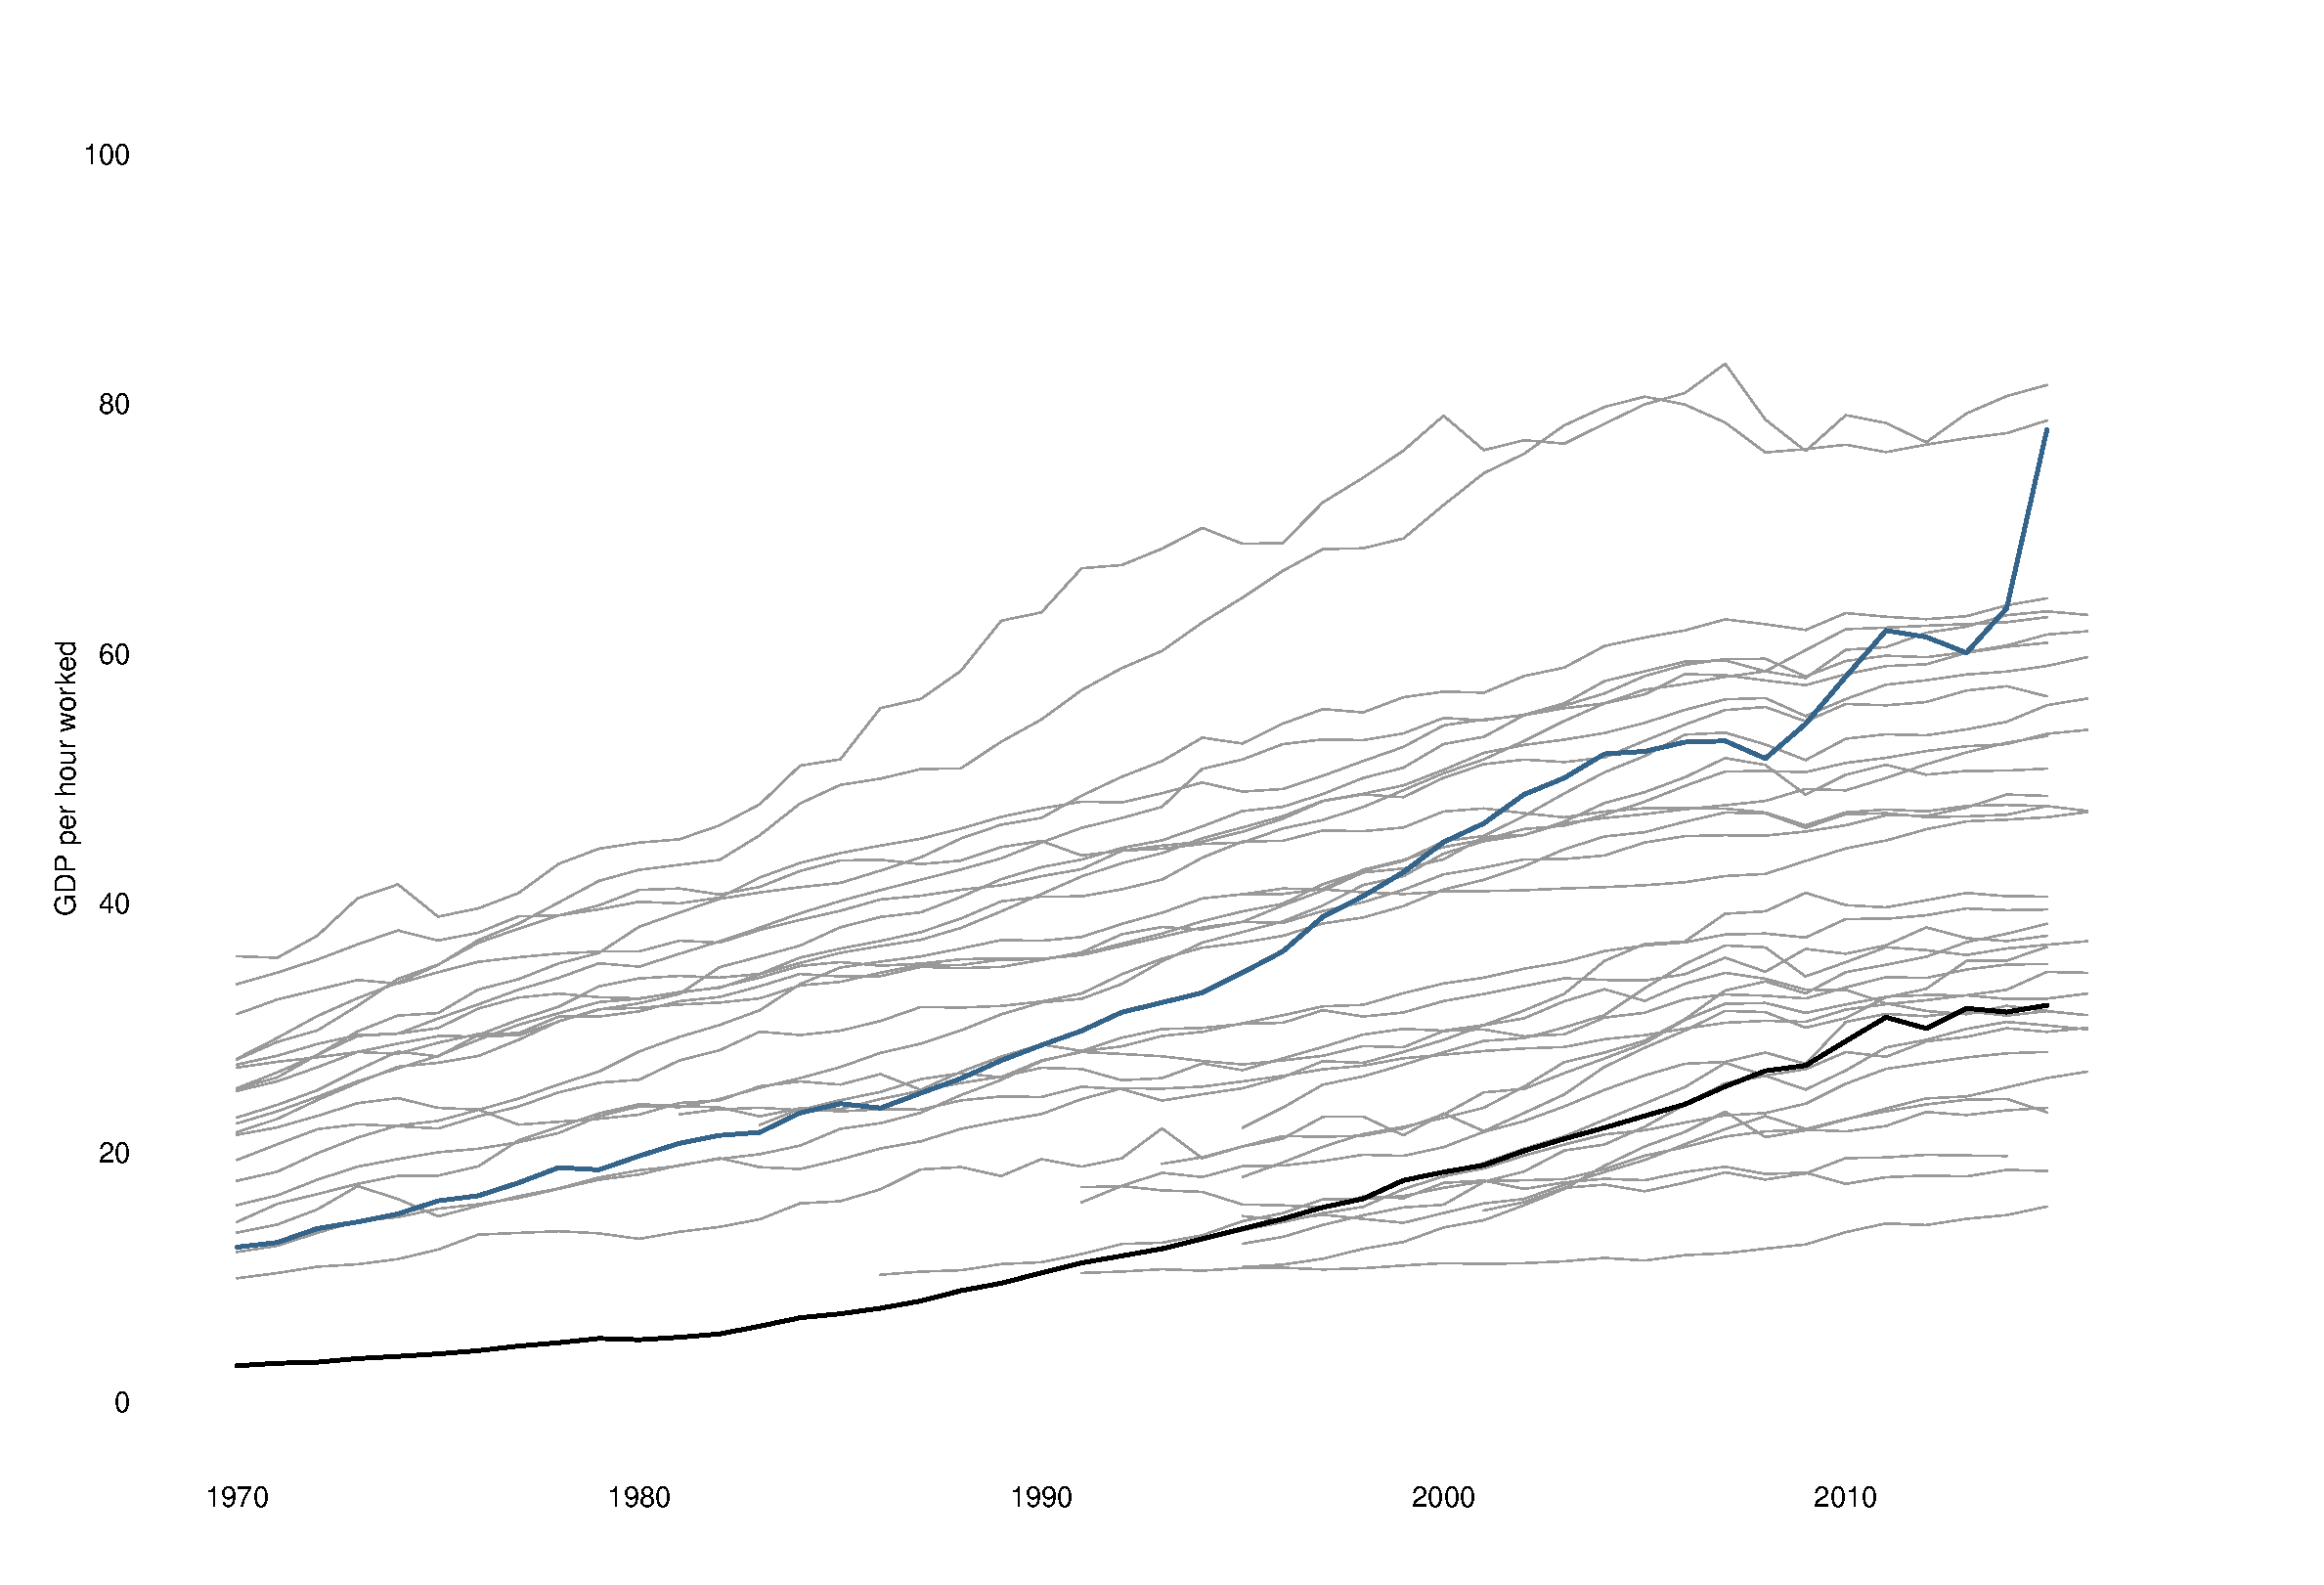
\includegraphics[scale=.3]{productivity.eps}
  \end{figure}
\end{frame}
%--------------------------------------

%--------------------------------------
\begin{frame}
 The Cobb-Douglas model shows that there are three potential ways through which to increase productivity
\begin{enumerate}
  \item $L$: Increase in labour force  
  \item $K$: Increasing the amount of capital per worker (capital deepening)
  \item $A$: Improving the efficiency of the economy (technological progress)  
\end{enumerate}
\end{frame}
%--------------------------------------

%--------------------------------------
\begin{frame}
 Increasing the labour will add to growth if 
 \begin{align}
   \alpha+\beta>1
 \end{align}
 \medskip
 i.e. under increasing returns to scale; most growth theories assume constant returns to scale (CRS)
 \begin{align}
   \alpha+\beta &= 1\\
   \frac{Y_t}{L_t} &= A_t \left(\frac{K_t}{L_t}\right)^{\alpha}
 \end{align}
\end{frame}
%--------------------------------------


%--------------------------------------
\begin{frame}
  Let's examine what determines growth under the CRS assumptions, given   
  \begin{align}
   \alpha+\beta &= 1
  \end{align}
  We get
  \begin{align}
    Y_t=A_tK^{\alpha}_tL^{1-\alpha}_t
  \end{align}
  \medskip
  Time is assumed to be continuous
  \begin{itemize}
    \item $t$ evolves smoothly instead of taking integer values like $t=1,t=2,...$.
  \end{itemize}
  \medskip
  The growth rate of $Y_t$ can be denoted by $G^Y_t$ and defined as
  \begin{align}
    G^Y_t=\frac{1}{Y_t}\frac{dY_t}{dt}
  \end{align}
  i.e growth equals the change in output divided by output level.
\end{frame}
%--------------------------------------

%--------------------------------------
\begin{frame}
  Can differentiate production function with respect to time; expressing it as a function of $G^Y_t$.
  E.g. for capital 
  \begin{align}
    \frac{\partial K_t^{\alpha}}{\partial t} &= \frac{\partial K_t^{\alpha}}{\partial K_t}\frac{\partial K_t}{\partial t} =\alpha K_t^{\alpha-1}\frac{\partial K_t}{\partial t}
  \end{align}
\end{frame}
%--------------------------------------

%--------------------------------------
\begin{frame}
  We can apply this for the whole function using the product rule
  \begin{align}
  \frac{\partial ABC}{\partial x}=BC\frac{\partial A}{\partial x}+AC\frac{\partial B}{\partial x}+AB\frac{\partial C}{\partial x}
\end{align}
\end{frame}
%--------------------------------------

%--------------------------------------
\begin{frame}
 Can calculate the terms involving the impact of changes in capital and labour inputs as
  \begin{align}
    \frac{\partial Y_t}{\partial t} &= \frac{\partial A_tK_t^{\alpha}L_t^{1-\alpha}}{\partial t}\\ \nonumber
    &= K_t^{\alpha}L_t^{1-\alpha}\frac{\partial A_t}{\partial t} + A_tL_t^{1-\alpha}\frac{\partial K_t^{\alpha}}{\partial t} + A_tK_t^{\alpha}\frac{\partial L_t^{1-\alpha}}{\partial t}\\ \nonumber
    &= K_t^{\alpha}L_t^{1-\alpha}\frac{\partial A_t}{\partial t} + \alpha A_tK_t^{\alpha-1}L_1^{1-\alpha} \frac{\partial K_t}{\partial t}  + (1-\alpha)A_tK_t^{\alpha}L_t^{-\alpha}\frac{\partial Lt}{\partial t}
  \end{align}
\end{frame}
%--------------------------------------

%--------------------------------------
\begin{frame}
 Calculate growth rate of output by dividing both sides by $Y_t$   
  \begin{align}
    \frac{1}{Y_t}\frac{\partial Y_t}{\partial t} & = \frac{K_t^{\alpha}L_t^{1-\alpha}}{A_tK_t^{\alpha}L_t^{1-\alpha}} \frac{\partial A_t}{\partial t} + \\ \nonumber & \alpha \frac{A_tK_t^{\alpha-1}L_1^{1-\alpha}}{A_tK_t^{\alpha}L_t^{1-\alpha}} \frac{\partial K_t}{\partial t} + (1-\alpha) \frac{A_tK_t^{\alpha}L_t^{-\alpha}}{A_tK_t^{\alpha}L_t^{1-\alpha}} \frac{\partial Lt}{\partial t}\\ \nonumber
    \frac{1}{Y_t}\frac{\partial Y_t}{\partial t} & = \frac{1}{A_t}\frac{\partial A_t}{\partial t} + \alpha \frac{1}{Kt}\frac{\partial K_t}{\partial t} + (1-\alpha) \frac{1}{L_t}\frac{\partial L_t}{\partial t}\\  
    G_t ^Y &=G_t^A +\alpha G_t^K + (1-\alpha)G_t^L
\end{align}
  \medskip
  NB- This is the same as dividing by $A_tK_t^{\alpha}L_t^{1-\alpha}$
\end{frame}
%--------------------------------------

%--------------------------------------
\begin{frame}
  \begin{align}
    G_t ^Y &=G_t^A +\alpha G_t^K + (1-\alpha)G_t^L
  \end{align}
  i.e. output growth equals technology growth plus a weighted average of the growth rates of capital and labour
  \begin{itemize}
    \item Weight determined by $\alpha$
  \end{itemize}
  \medskip
  This is the key equation in growth accounting studies. 
\end{frame}
%--------------------------------------

%--------------------------------------
\begin{frame}
  Growth accounting studies provide estimates of how much GDP growth over a certain time span is determined by 
  \begin{enumerate}
    \item Growth in the number of workers
    \item Growth in capital stock
    \item Improvement in Total Factor Productivity
  \end{enumerate}
\end{frame}
%--------------------------------------

%--------------------------------------
\begin{frame}
Calculating the growth equation
\begin{align}
  G_t ^Y &=G_t^A +\alpha G_t^K + (1-\alpha)G_t^L
\end{align}
\medskip
requires
\begin{itemize}
  \item A measure for output i.e. GDP
  \item Number of workers
  \item Capital stock estimate 
  \item Value for Total Factor Productivity
\end{itemize}
\end{frame}
%--------------------------------------

%--------------------------------------
\begin{frame}
One empirical issue is that the value for TFP ($A_t$) can't be directly observed. 
However, if we know the value of parameter $\alpha$ we can get an estimate for growth. 
\begin{align}
  G_t ^A &=G_t^Y -\alpha G_t^K - (1-\alpha)G_t^L
\end{align}
\end{frame}
%--------------------------------------

%--------------------------------------
\begin{frame}
  Solow (1957) pointed out that an $\alpha$ estimate could be obtained by looking at the shares of GDP paid to workers and to capital. 
  To illustrate, consider a perfectly competitive firm that is seeking to maximise profits and the firm
  \begin{itemize}
    \item Sells product at price $P_t$
    \item Pays wages $W_t$
    \item Rents its capital at a rate of $R_t$
  \end{itemize}
\end{frame}
%--------------------------------------

%--------------------------------------
\begin{frame}
  The firm's profits are given by
  \begin{align}
    \Pi_t &= P_tY_t - R_tK_t -W_tL_t\\ \nonumber
    &= P_tA_tK_t^{\alpha}L_t^{1-\alpha}-R_tK_t - W_tL_t  
  \end{align}
  $P_t Y_t$ is total nominal GDP\\
  $R_t K_T$ is the total amount of income paid to capital\\
  $W_t L_t$ is the total amount of income paid to wages  
\end{frame}
%--------------------------------------

%--------------------------------------
\begin{frame}
  The firm only needs to decide how much labour and capital to use
  It will therefore maximise profits by differentiating the function with respect to capital and labour and set the derivatives equal to zero which provides two conditions
\begin{align}
  \frac{\partial \Pi_t}{\partial K_t} &= \alpha P_tA_tK_t^{\alpha-1}L_t^{1-\alpha} -R_t\\ \nonumber
  & = \alpha \frac{P_tY_t}{K_t} - R_t = 0\\ 
  \frac{\partial \Pi_t}{\partial L_t} &= (1-\alpha) P_tA_tK_t^{\alpha}L_t^{-\alpha} - W_t \\ \nonumber
  & = (1-\alpha) \frac{P_tY_t}{L_t}- W_t = 0
\end{align}
\end{frame}
%--------------------------------------

%--------------------------------------
\begin{frame}
Rearranging we get
\begin{align}
  \alpha &= \frac{R_tK_t}{P_tY_t}\\ 
  1-\alpha &= \frac{W_tL_t}{P_tY_t}
\end{align}
\medskip
$\alpha$ will be the total amount of income paid to capital relative to total income, at the aggregate level nominal GDP
\begin{itemize}
  \item $1-\alpha$ can be calculated as the fraction of income paid to workers instead of compensating capital.
\end{itemize}
\end{frame}
%--------------------------------------

%--------------------------------------
\begin{frame}
 Solow's results implied that $\alpha<0.5$
  \begin{itemize}
    \item For most countries the national income accounts show that wage income explain most of GDP
    \item $\alpha=\frac{1}{3}$ is used, based on the estimates for the US economy
  \end{itemize}
  \medskip
  Solow's paper also concluded that capital deepening had not been that important for US growth
  \begin{itemize}
    \item TFP growth accounted for 87.5\% of growth in productivity over the period    
  \end{itemize}
  \medskip
  TFP is sometimes called the Solow residual because it is a backed out calculation that makes things add up
\end{frame}
%--------------------------------------

%--------------------------------------
\begin{frame}
In the standard Swan-Solow model the production functions links output to capital and labour inputs as well as a technological efficiency parameter.
\begin{align}
  Y_t = AF(K_t,L_t) 
\end{align}
\medskip
A key feature of the model is that, with a constant labour supply, there are diminishing marginal returns to capital accumulation meaning that each increase in capital will give a progressively smaller increase in output
\begin{align}
  \frac{\delta^2Y_t}{\delta K_t}<0
\end{align}
\end{frame}
%--------------------------------------

%--------------------------------------
\begin{frame}
 Some additional assumptions of the model  
  \begin{align}
    Y_t =C_t+I_t\\ 
    S_t=Y_t-C_t=I_t \\ 
    \frac{\partial K_t}{\partial t}=I_t -\delta K_t \\
    S_t=sY_t
  \end{align}
  \medskip
  i.e. 
  \begin{itemize}
    \item All output takes the form of consumption or investment 
    \item Savings will equal investment
    \item Capital will depreciate
    \item Consumers save constant share of income
  \end{itemize}
\end{frame}
%--------------------------------------

%--------------------------------------
\begin{frame}
  These assumptions tell us something about the model's capital dynamics since the amount of savings equals the amount of investment, this means that investment is also a constant fraction of output
  \begin{align}
    I_t=sY_t
  \end{align}
  This entails that the capital stock changes over time according to
  \begin{align}
    \frac{\partial K_t}{\partial t}=sY_t-\delta K_t
  \end{align}
\end{frame}
%--------------------------------------

%--------------------------------------
\begin{frame}
    Capital stock development over time depends on whether investments are greater, equal to, or less than the depreciation rate
 \begin{align}
    \partial K_t < sY_t &\Rightarrow \frac{\partial K_t}{\partial t} > 0\\
    \partial K_t = sY_t &\Rightarrow \frac{\partial K_t}{\partial t} = 0\\
    \partial K_t > sY_t &\Rightarrow \frac{\partial K_t}{\partial t} < 0
 \end{align}
 \medskip
 The stock of capital will stay constant if the capital/output ratio is
  \begin{align}
    \frac{K_t}{Y_t} = \frac{s}{\delta}
  \end{align}
\end{frame}
%--------------------------------------

%--------------------------------------
\begin{frame}
  The level of investments is given by
\begin{align}
  I_t=sY_t=sAF(K_t,L_t)
\end{align}
 This means that an one-off increase in technology level $A$ has the same effect as a one off increase in $s$
 \begin{itemize}
   \item Capital and output gradually increase to a new level
 \end{itemize}
\end{frame}
%--------------------------------------

%--------------------------------------
\begin{frame}
  The model implies a very important difference between these two determinants of growth
  \begin{itemize}
    \item Savings rate $s$ is subject to a limit, whereas as $A$ does not face such constraints    
  \end{itemize}
  \medskip
  Therefore, in order to have long-term sustainable growth increases in TFP matter
  \begin{itemize}
    \item Specifically, growth through capital accumulation will taper off over time producing a one-off increase in output per worker whereas TFP growth can lead to sustained higher growth rates of output per worker 
  \end{itemize}  
\end{frame}
%--------------------------------------

%--------------------------------------
\begin{frame}
  We can define the capital-output ratio as
\begin{align}
  \frac{K_t}{Y_t}=K_tY_t^{-1}=x_t
\end{align}
\medskip
and the growth rate can be written as
\begin{align}
  \frac{\Delta x_t}{x_t} = \frac{\Delta K_t}{K_t} - \frac{\Delta Y_t}{Y_t}
\end{align}
\end{frame}
%--------------------------------------

%--------------------------------------
\begin{frame}
  We can now define the growth equation 
\begin{align}
  G^Y_t &= G^A_t + \alpha G^K_t + (1-\alpha)G^L_t  
\end{align}
as
\begin{align}
  \frac{\Delta Y_t}{Y_t} &= g + \alpha \frac{\Delta K_t}{K_t} + (1-\alpha)n
\end{align}

Capital growth is given as
\begin{align}
  \frac{\Delta K_t}{K_t} = s \frac{Y_t}{K_t} - \delta = \frac{s}{x_t}-\delta
\end{align}

Meaning that the growth of the capital-output ratio is given by
\begin{align}
  \frac{\Delta x_t}{x_t} &= (1-\alpha) \frac{\Delta K_t}{K_t} -g - (1-\alpha)n\\ \nonumber
                         &= (1-\alpha) (\frac{s}{x_t} - \frac{g}{1-\alpha}-n-\delta)
\end{align}
\end{frame}
%--------------------------------------

%--------------------------------------
\begin{frame}
  The growth rate of $x_t$ depends negatively on the value of $x_t$
  \begin{itemize}
    \item When it is above a certain $x_t$ value the growth rate will decline and it will increase under said $x_t$ value
  \end{itemize}
  \medskip
  The capital-output ratio therefore exhibits convergent dynamics leading to a particular long-run steady state value. 
  In equilibrium the capital-output ratio equals 0, this is when
  \begin{align}
    x^* = \frac{s}{\frac{g}{1-\alpha}+n+\delta}
    \end{align}
\end{frame}
%--------------------------------------

%--------------------------------------
\begin{frame}
 \textbf{NB-} Results from growth accounting studies can potentially be misleading as they misidentify the source of growth
 \begin{itemize}
   \item Consider a country that allocates a fixed share of GDP to investments but is experiencing a steady growth in TFP
   \item The Swan-Solow model predicts in this case a steady increase in output per worker and an increase in capital stock
   \item Observing this increase a growth accounting study might conclude that a certain percentage of growth is caused by capital accumulation, whereas all growth is caused by the TFP
 \end{itemize}
\end{frame}
%--------------------------------------

%--------------------------------------
\begin{frame}
  \begin{figure}
    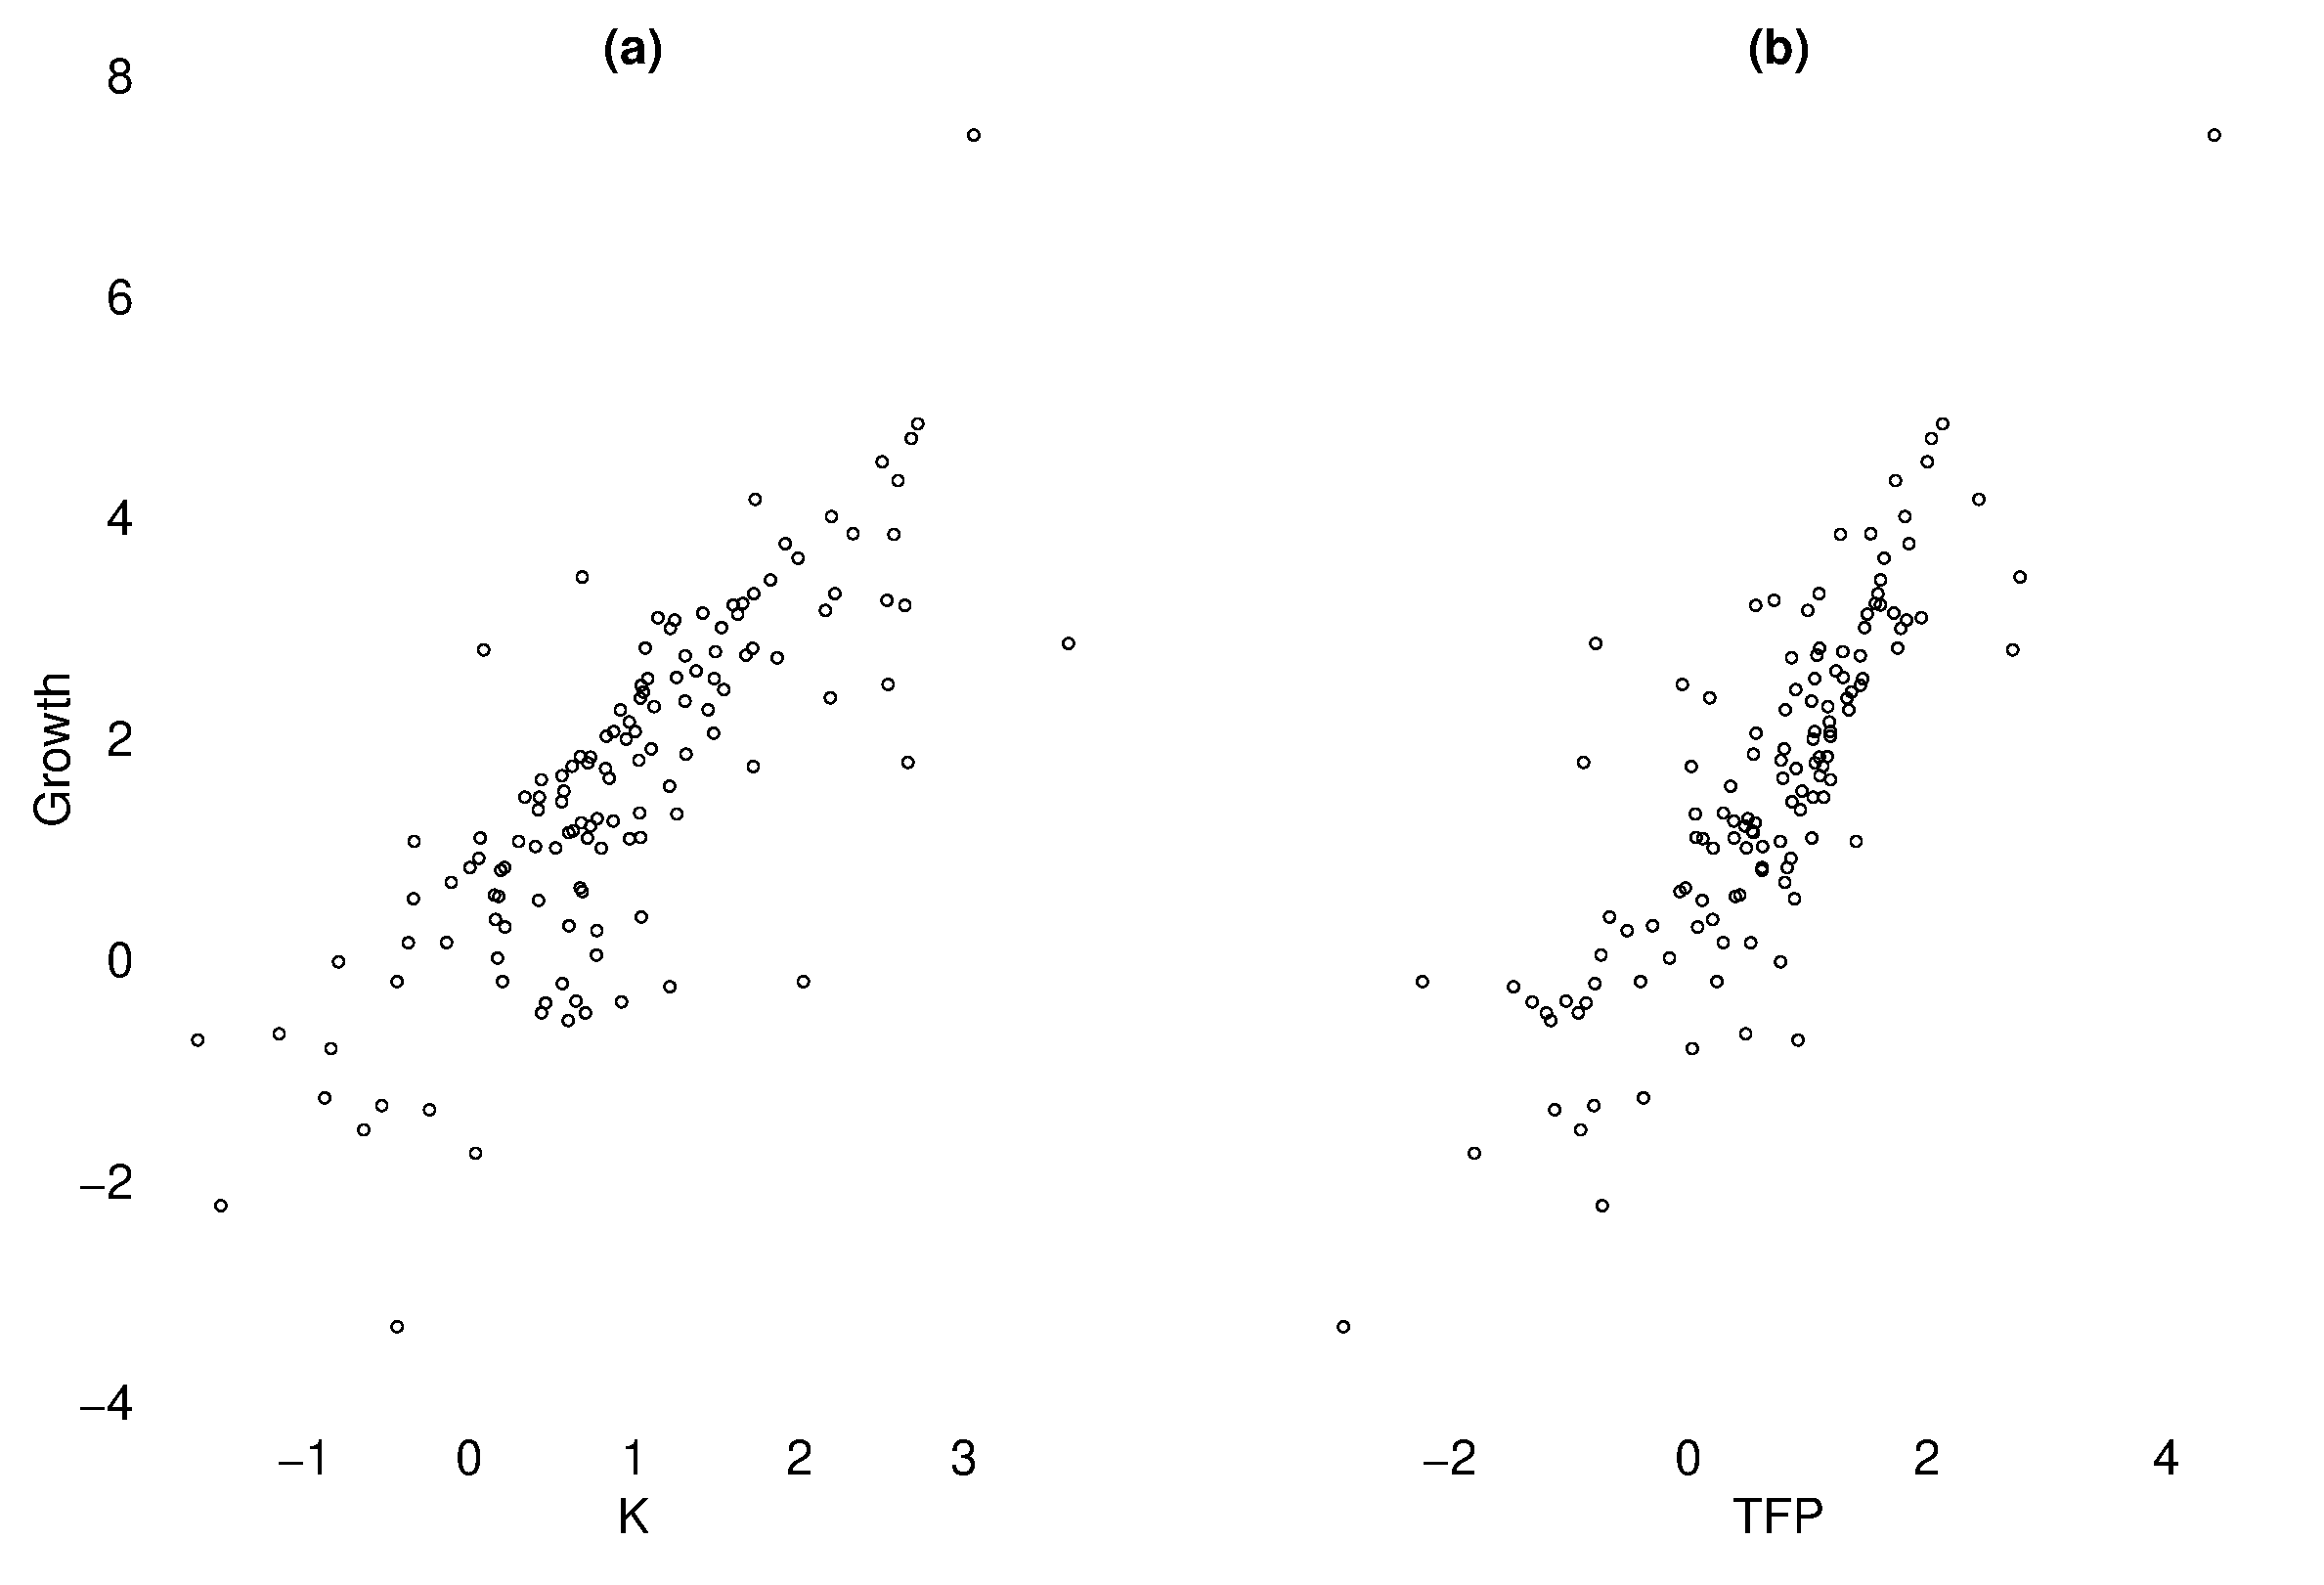
\includegraphics[scale=.3]{growth.eps}
  \end{figure}
\end{frame}
%--------------------------------------

%--------------------------------------
\begin{frame}
  \begin{figure}
    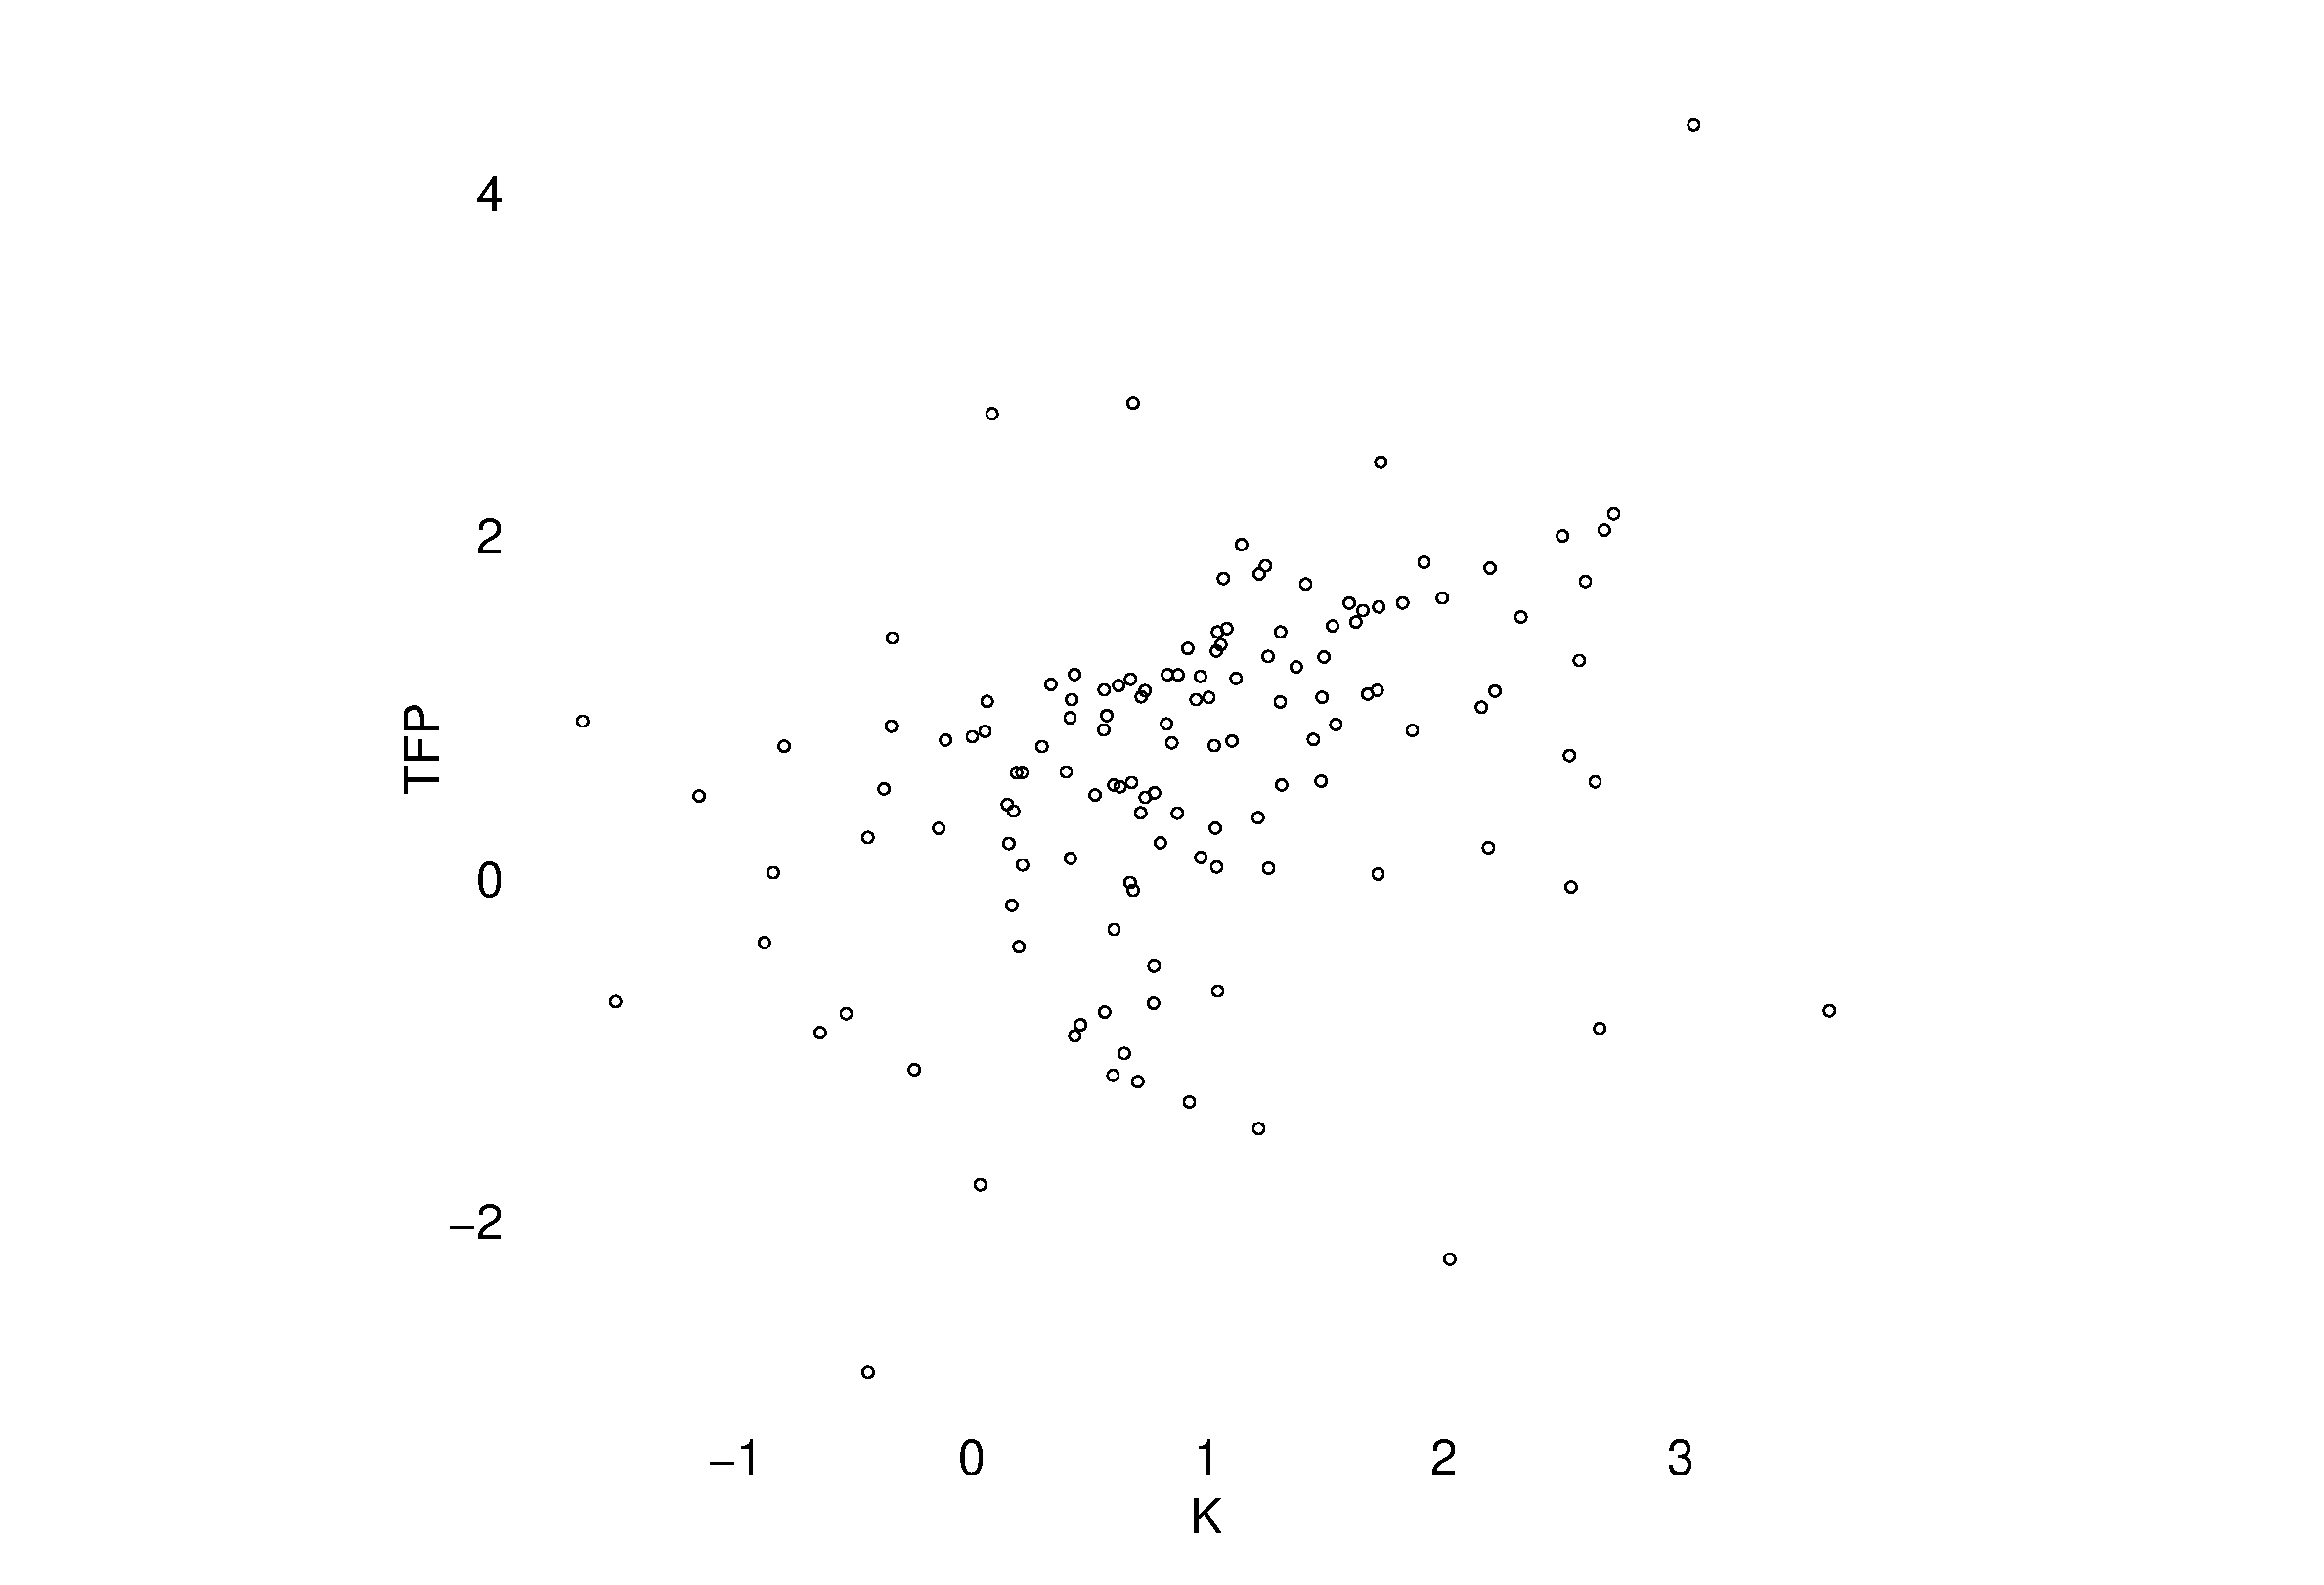
\includegraphics[scale=.3]{growth2.eps}
  \end{figure}
\end{frame}
%--------------------------------------


%--------------------------------------
\begin{frame}
 One main challenge for future economic growth in Europe is dealing with demographic changes
 \begin{itemize}
   \item Specifically the aging of the population
   \item Population growth is slowing and will peak in the middle of the century
   \item Worryingly, the working population (15-64 year) has already peaked and will decline
 \end{itemize}
   \medskip
   Macroeconomic problems facing Europe are twofold
   \begin{enumerate}
     \item Short term: weak aggregate demand and high level of debt
     \item Long term: Changing demography 
   \end{enumerate}
\end{frame}
%--------------------------------------

%--------------------------------------
\begin{frame}
  \begin{figure}
    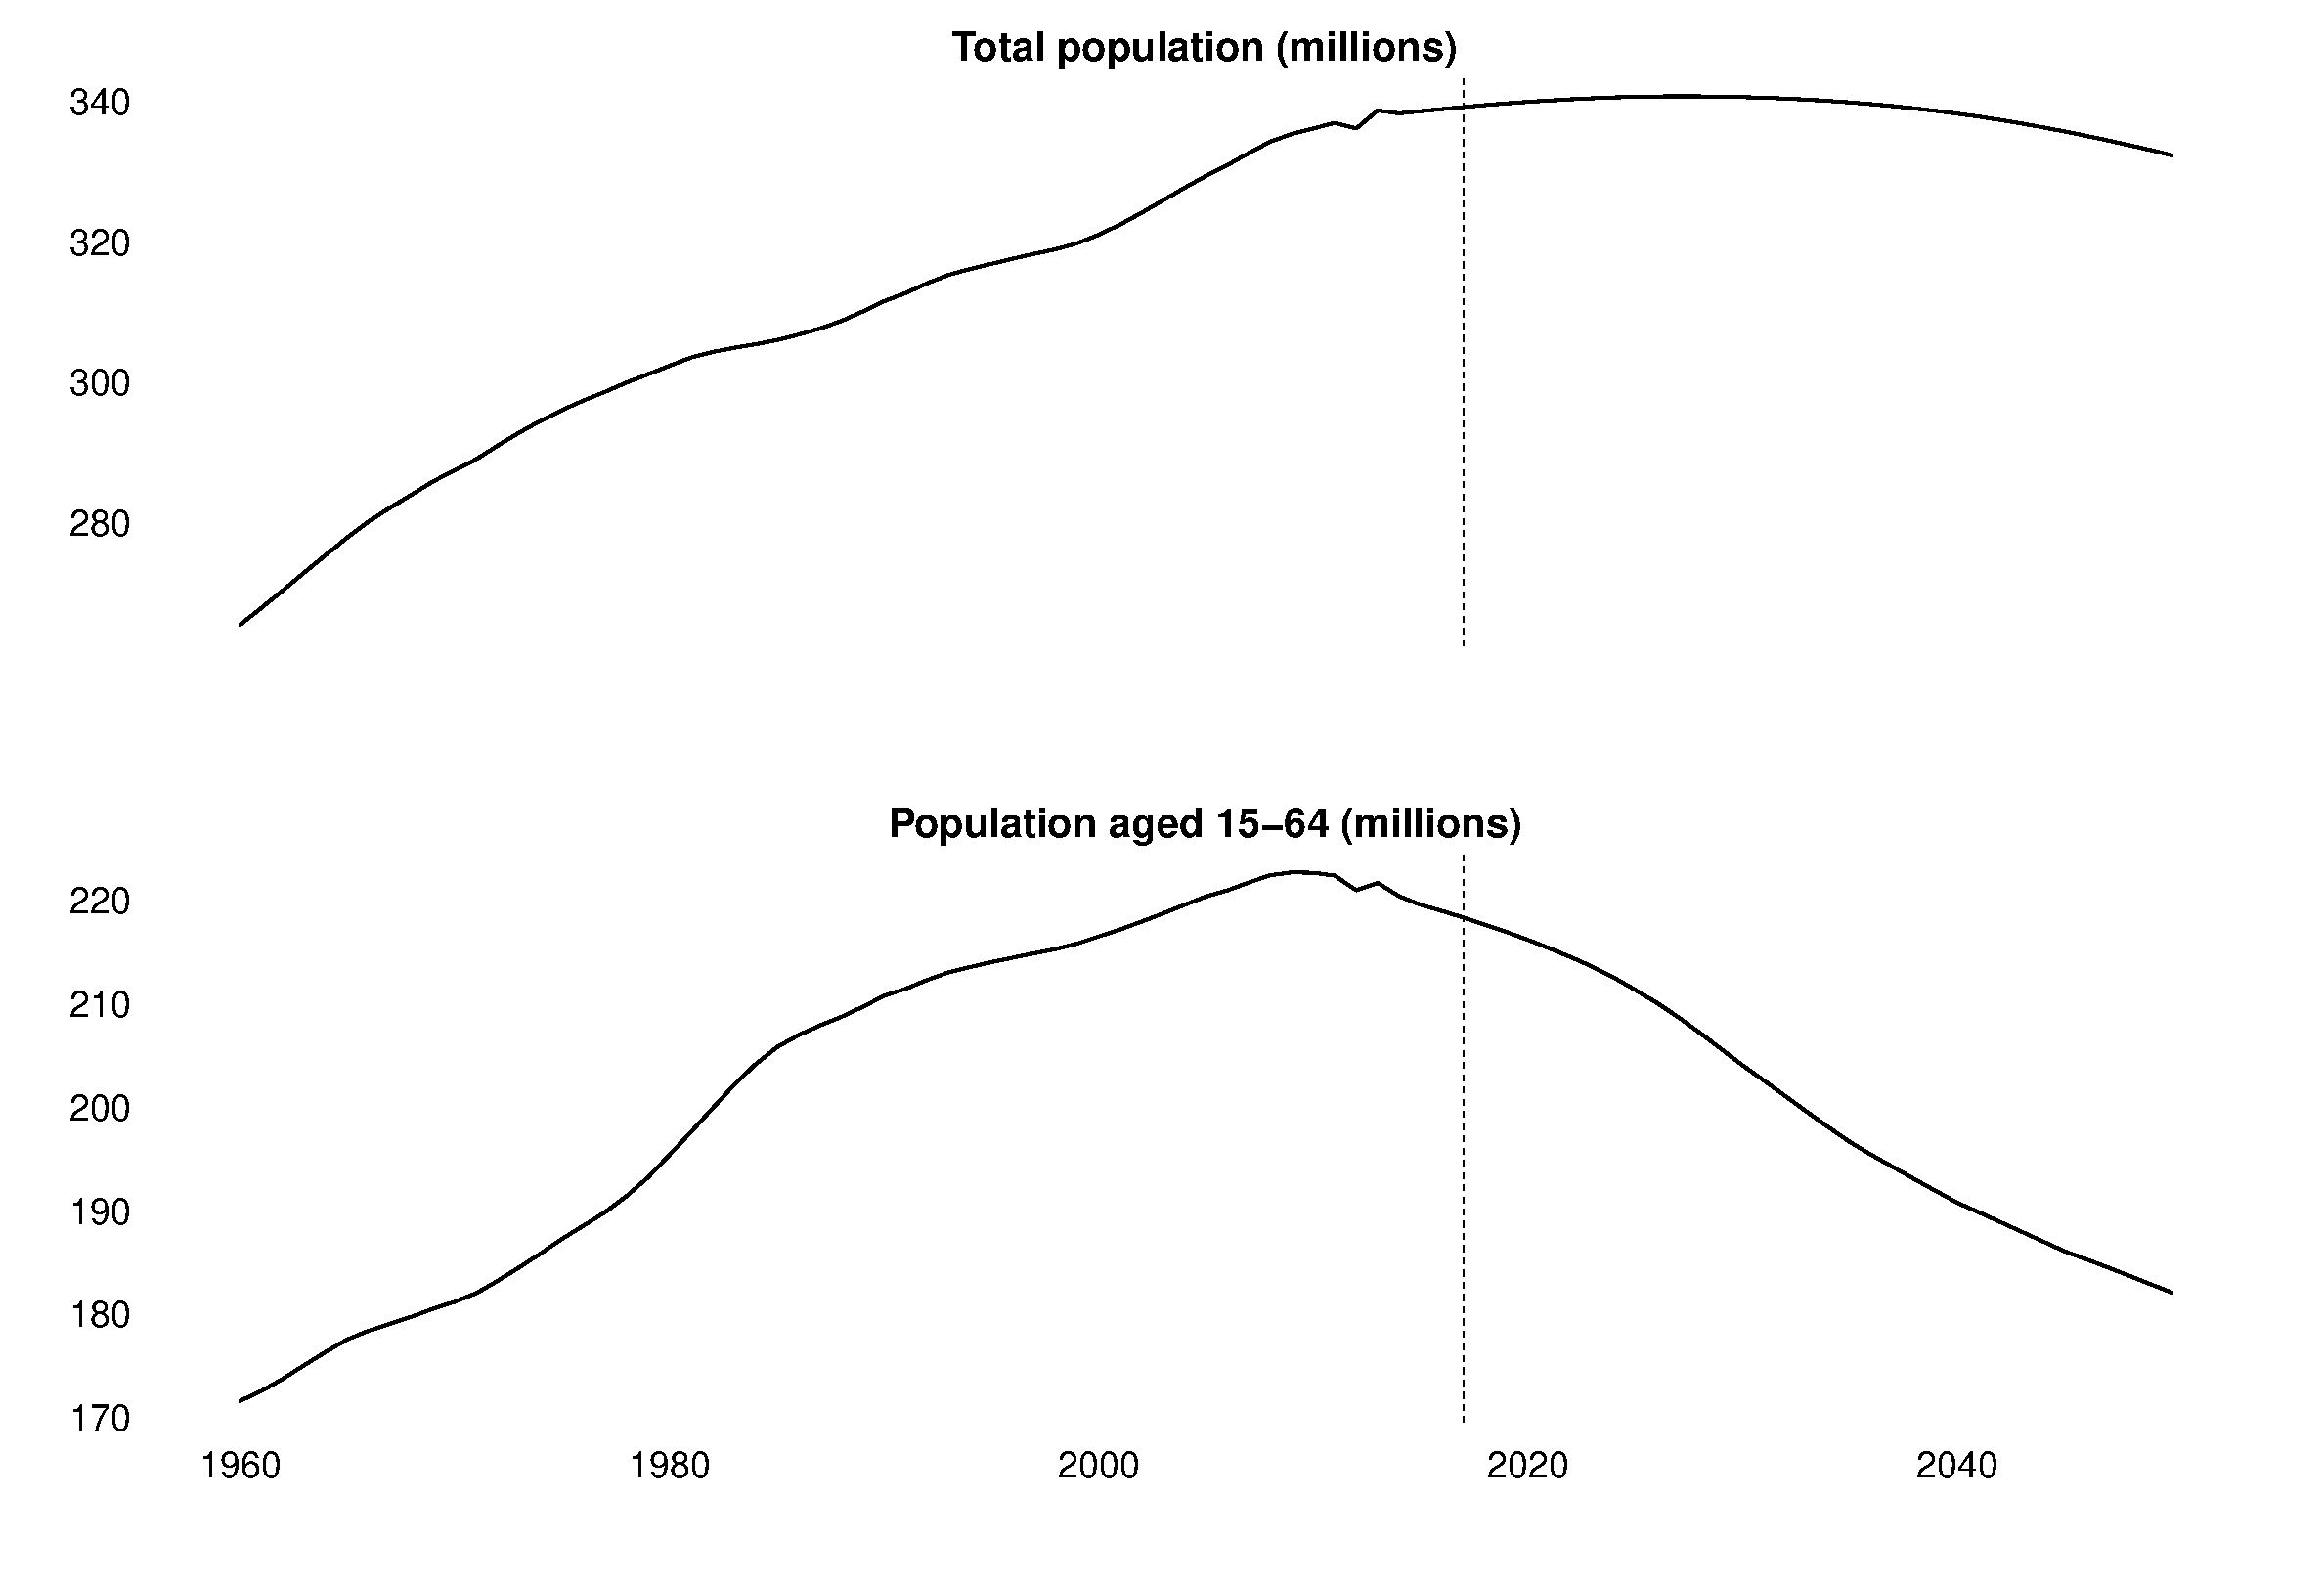
\includegraphics[scale=.3]{population_projection.eps}
  \end{figure}
\end{frame}
%--------------------------------------

%--------------------------------------
\begin{frame}
  \begin{figure}
    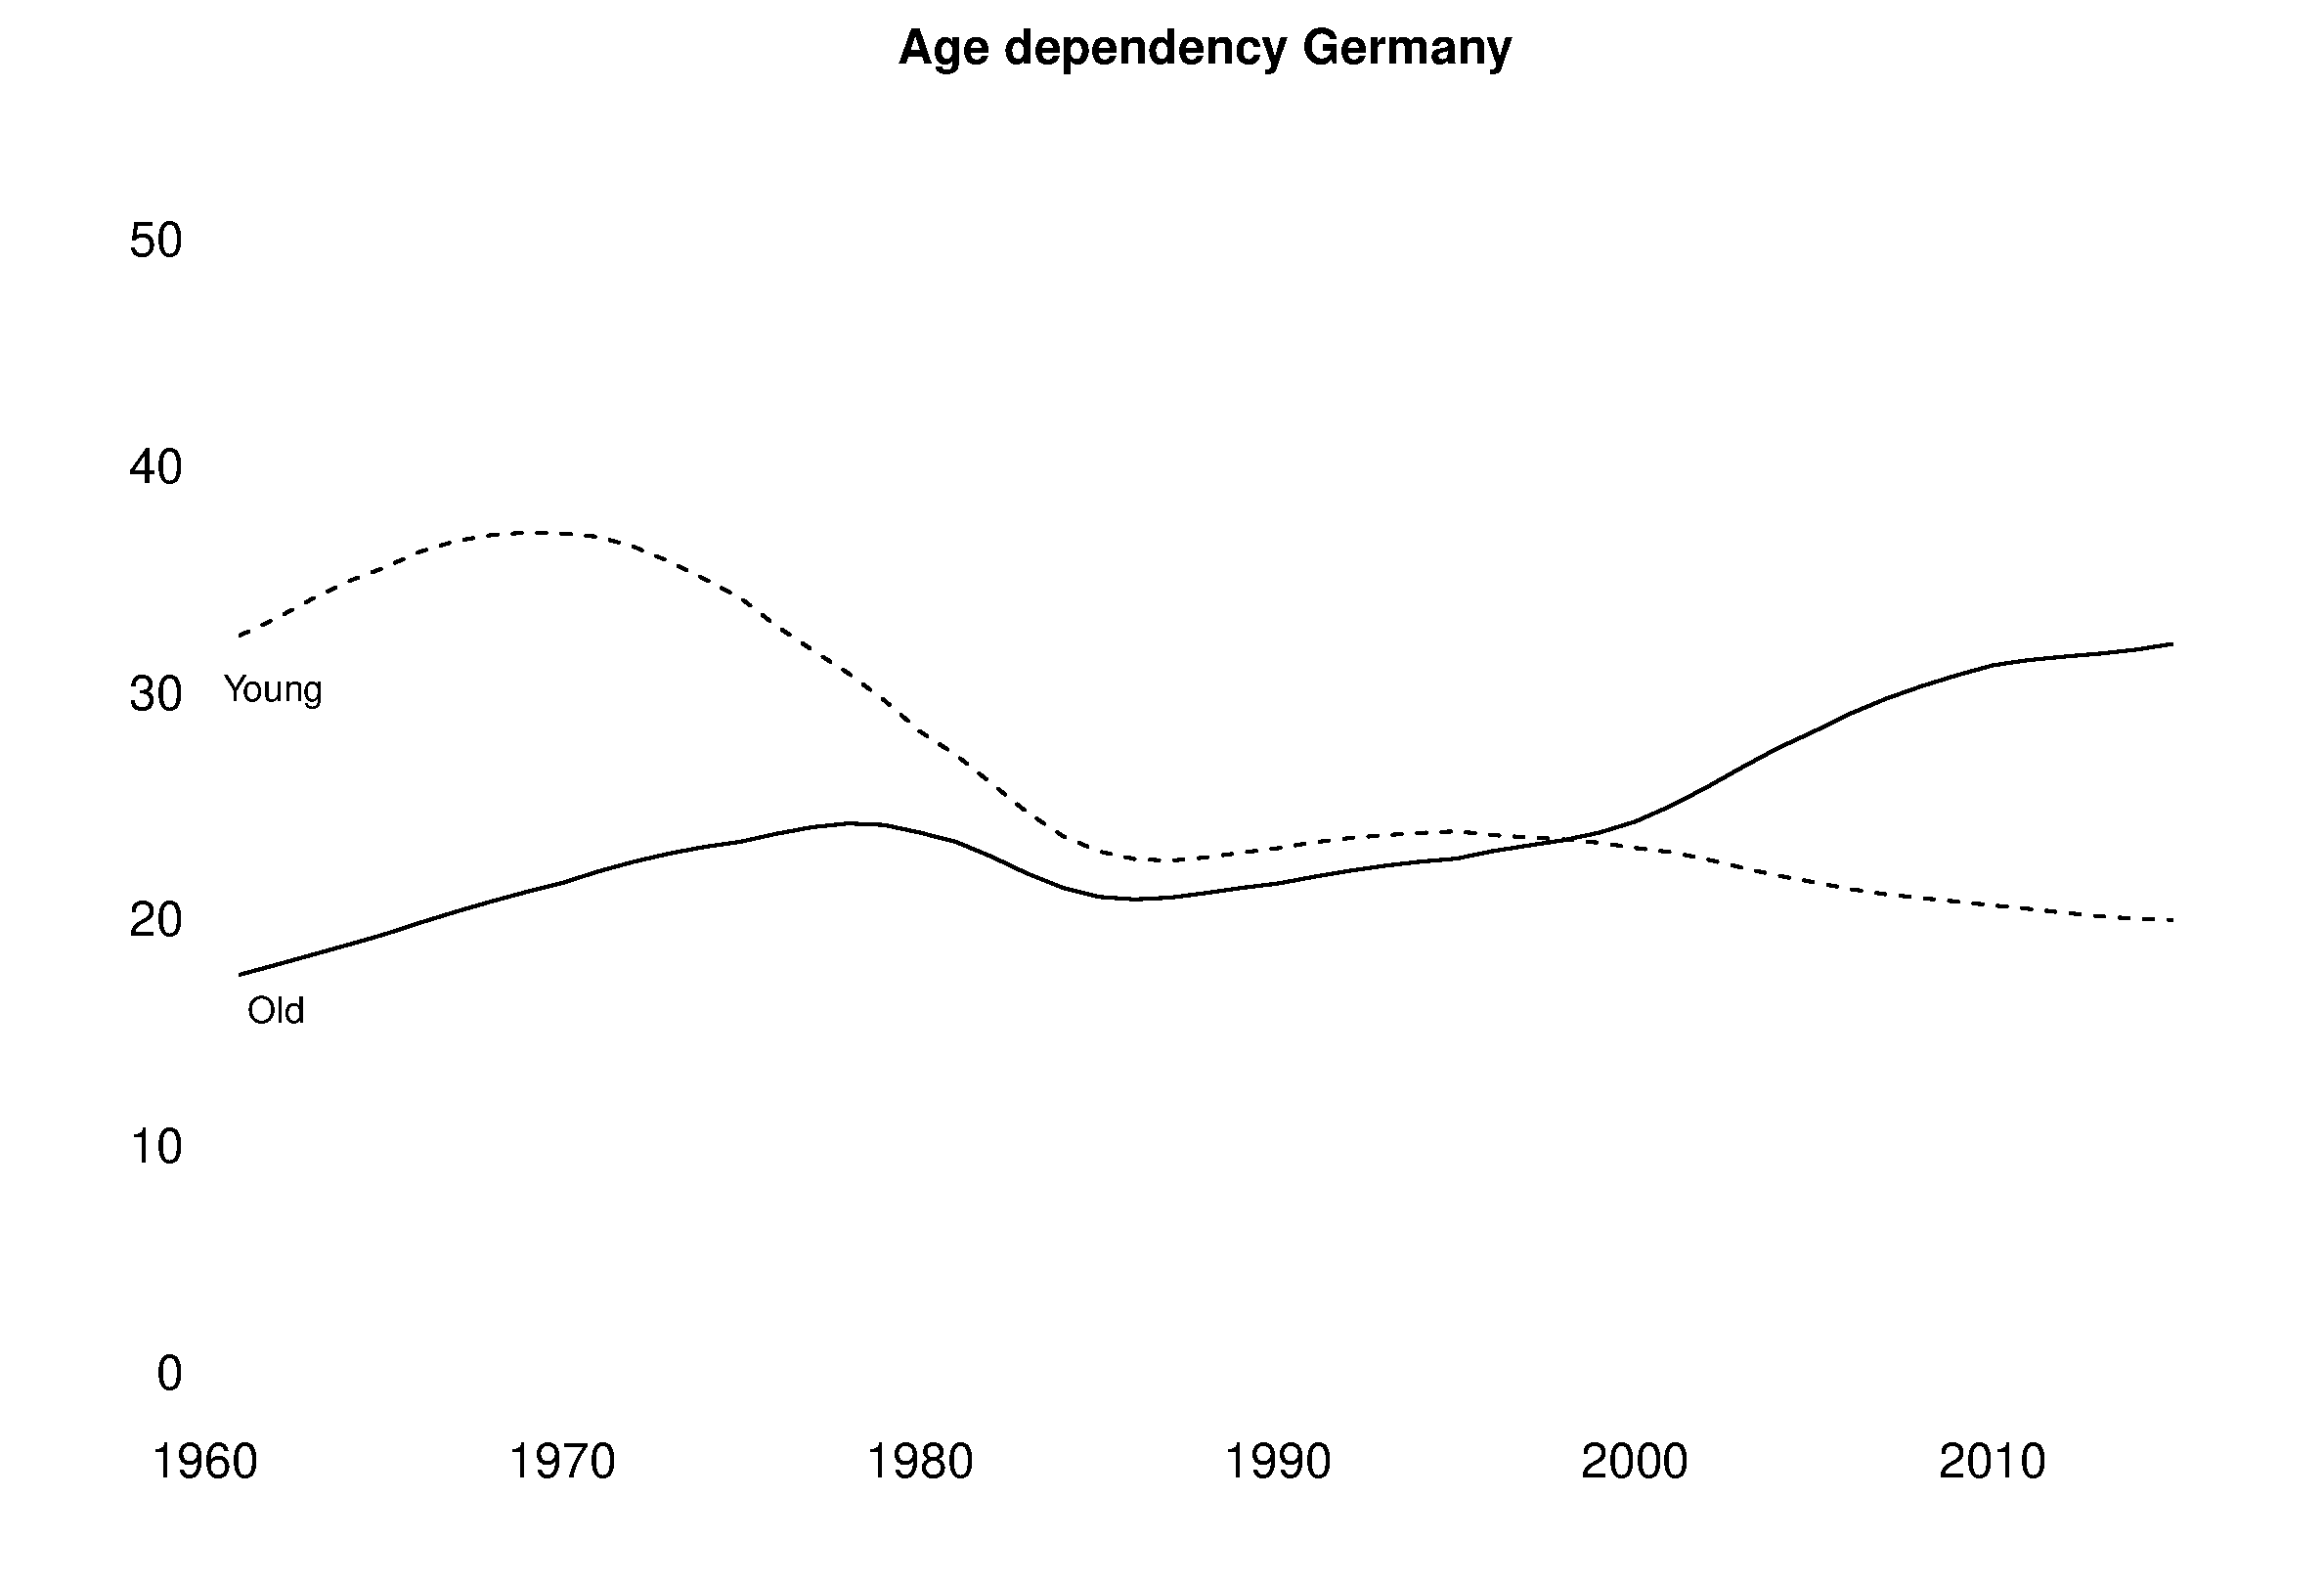
\includegraphics[scale=.3]{age_ger.eps}
  \end{figure}
\end{frame}
%--------------------------------------

%--------------------------------------
\begin{frame}
 Young (1992) provides a growth accounting study focusing on Hong Kong and Singapore
 \begin{itemize}
   \item Both cities have been very successful in restructuring their economy; Hong Kong experienced an economic growth of 147\% between the early 1970s and 1990; Singapore 154\%
 \end{itemize}
 \medskip
 Young focuses on these two cities as they have a similar background yet are different on a number of issues emphasized by growth theory. 
  Some similarities in the prewar period include
  \begin{itemize}
    \item Both British colonies
    \item Entrep\^{o}t trading ports
  \item Little domestic manufacturing
  \end{itemize}
\end{frame}
%--------------------------------------

%--------------------------------------
\begin{frame}
  \begin{figure}
    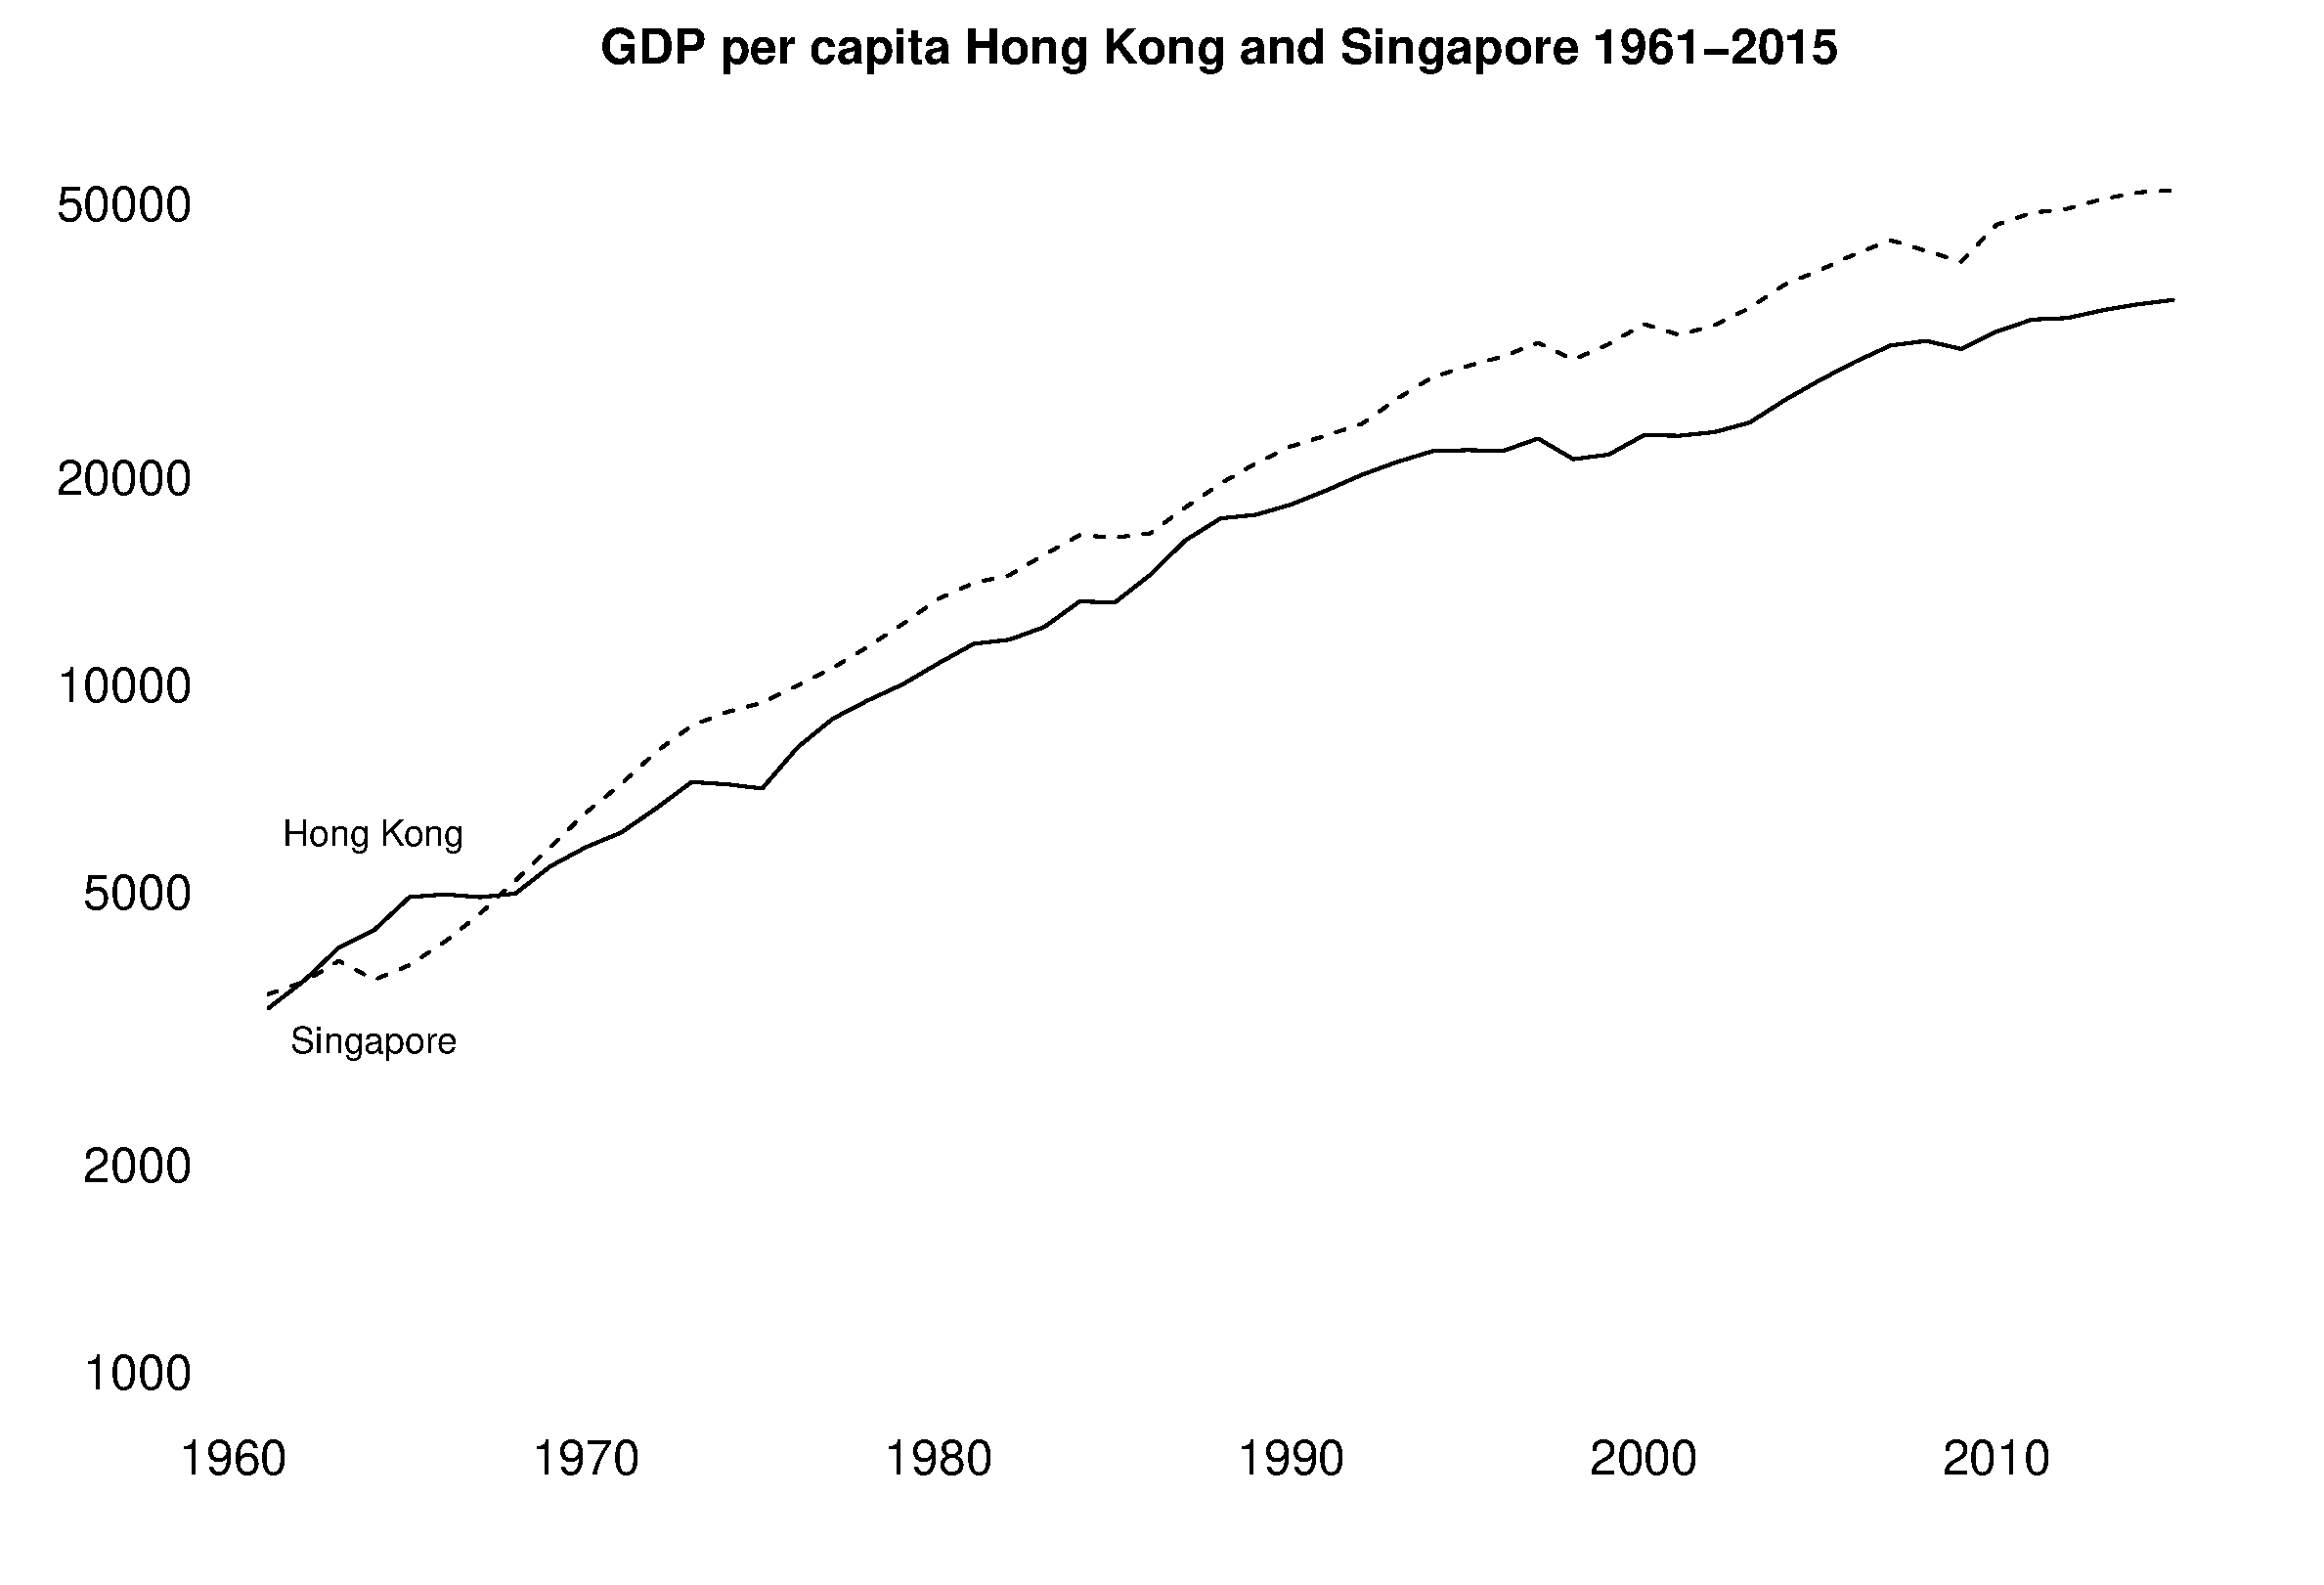
\includegraphics[scale=.3]{hongkong_singapore.eps}
  \end{figure}
\end{frame}
%--------------------------------------


%--------------------------------------
\begin{frame}
  During the postwar period, both city-states developed export-dependent manufacturing industries, going from producing textiles to clothing, plastics, electronics, and since the 1980s shifting to banking and financial services.
  Two important differences between the cities are
\begin{enumerate}
  \item Hong Kong had a better educated population in the early postwar years
  \item Hong Kong has pursuit laissez-faire policies, whereas Singapore implemented forced national savings and attracted a lot of foreign direct investment
\end{enumerate}
\end{frame}
%--------------------------------------

%--------------------------------------
\begin{frame}
  \begin{figure}
    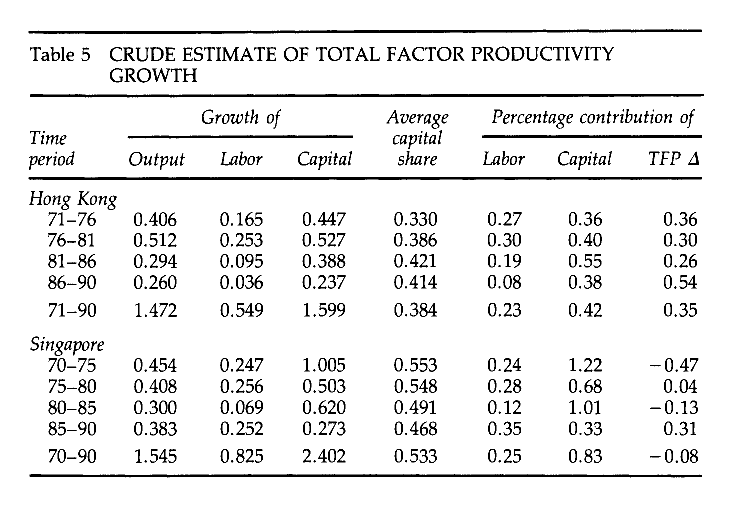
\includegraphics[scale=.8]{young.eps}
  \end{figure}
\end{frame}
%--------------------------------------

%--------------------------------------
\begin{frame}
  \begin{figure}
    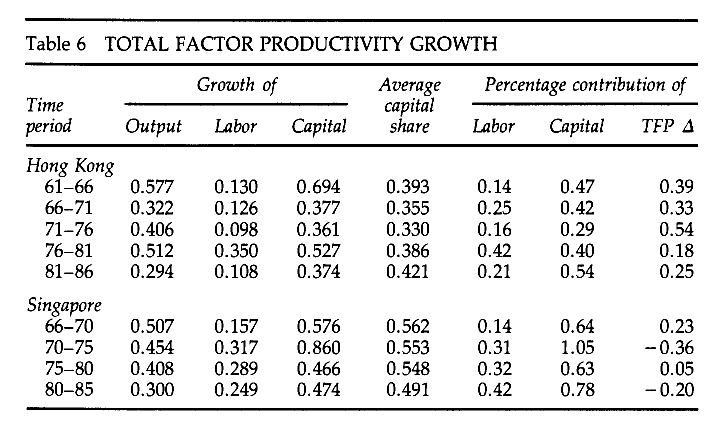
\includegraphics[scale=.8]{young2.eps}
  \end{figure}
\end{frame}
%--------------------------------------

%--------------------------------------
\begin{frame}
  Young finds that both cities experienced an economic transformation going roughly through the same industries
  \begin{itemize}
    \item Singapore seemed to have done this in a more compressed period
    \item Rate of structural transformation is 0.209 for Singapore, 0.082 for Hong Kong
    \item Structural transformation is here measured by the allocation of labour in across two-digit ISIC manufacturing sectors
  \end{itemize}  
\end{frame}
%--------------------------------------

%--------------------------------------
\begin{frame}
Important is the source of growth: Capital deepening or TFP growth
  \begin{itemize}
    \item TFP growth played important role in Hong Kong, contributing about 30 to 50\% to output growth, with an average of 35\% between 1971-1990
    \item In Singapore capital was key, contributing to 83\% of output growth (did not contribute to TFP growth)
  \end{itemize}
  \medskip
  One advantage of TFP growth over growth based on capital accumulation is that it is more sustainable over the long run.   
\end{frame}
%--------------------------------------


%--------------------------------------
\begin{frame}
Young provides a theoretical explanation for the different patterns across the two cities focusing on
\begin{enumerate}
  \item Innovations ($N$)
  \item Bounded learning by doing ($T$)
\end{enumerate}
This is to account for the fact that new technologies do not achieve their full productivity potential directly upon implementation but that there are gains made by continuous adjustments.
\end{frame}
%--------------------------------------

%--------------------------------------
\begin{frame}
  \begin{figure}
    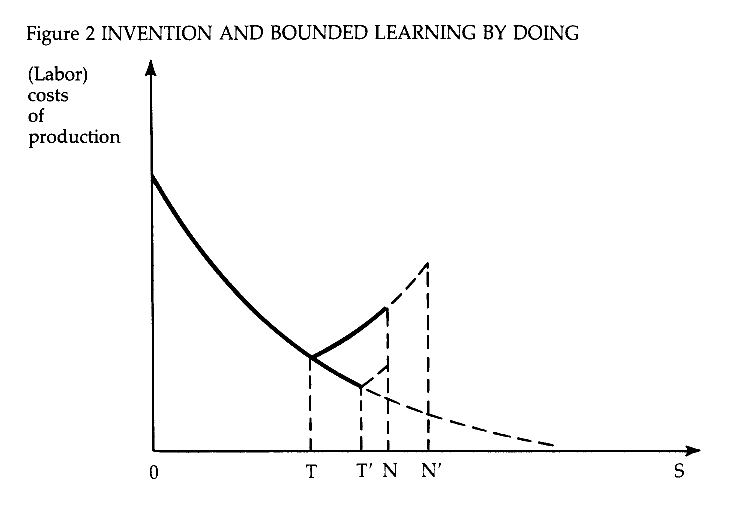
\includegraphics[scale=.8]{young3.eps}
  \end{figure}
\end{frame}
%--------------------------------------

%--------------------------------------
\begin{frame}
  \begin{figure}
    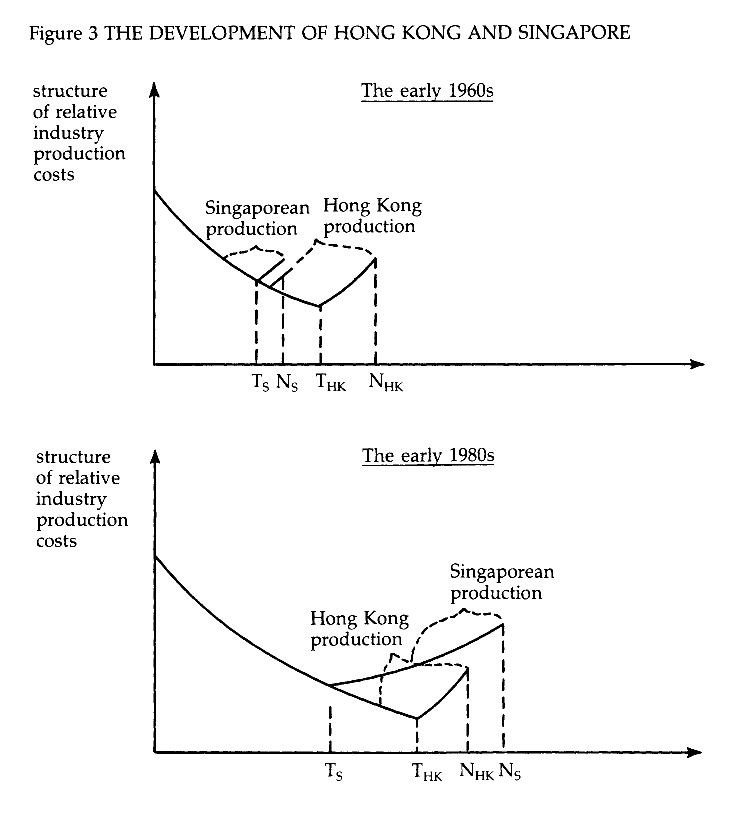
\includegraphics[scale=.7]{young4.eps}
  \end{figure}
\end{frame}
%--------------------------------------

%--------------------------------------
\begin{frame}
  Young argues that
\begin{itemize}
  \item In the early 1960s Hong Kong learning maturity was greater than that of Singapore: $T_{HK}>T_S$
  \item Hong Kong found it easier to copy technologies and enter new sectors: length of $[T_{HK},N_{HK}]$ relative to $[T_{S},N_{S}]$
  \item By the early 1980s Singapore had caught up, and both economies experienced substantial learning by doing: Rightward movement of $T_{HK},T_S$  
\end{itemize}
\end{frame}
%--------------------------------------

%--------------------------------------
\begin{frame}
  \begin{figure}
    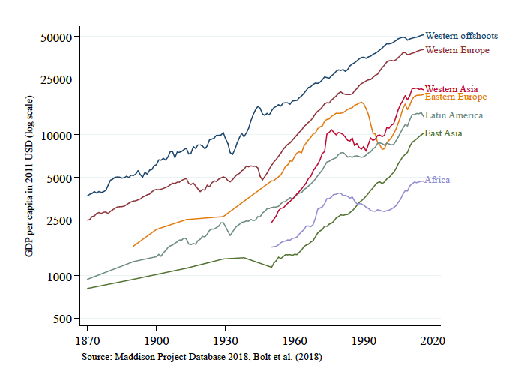
\includegraphics[scale=1.2]{bolt_et_al.eps}
  \end{figure}  
\end{frame}
%--------------------------------------

%--------------------------------------
\begin{frame}
  What matters for long-term growth?
  \begin{itemize}
    \item Demography
    \item Geography
    \item Institutions
    \item Natural resources
    \item War and conflict
    \item Trade
    \item Education
    \item Colonial history
    \item Macroeconomic policy
  \end{itemize}
\end{frame}
%--------------------------------------

%--------------------------------------
\begin{frame}
  Cross-country evidence on growth determinants is often discounted
  \begin{itemize}
    \item Major issue is that there are many candidate models and choice in variable selection leaves room for data mining
  \end{itemize}
  \medskip
  Ciccone \& Jarocinski (2010) examine the sensitivity of results to changes in data and variable selection using Bayesian Model Averaging
  \begin{itemize}
    \item They find that the results are very sensitive to measurement error in income estimates
  \end{itemize}  
\end{frame}
%--------------------------------------

%--------------------------------------
\begin{frame}
  Consider a dataset with $N$ countries, where $N$ is relatively large to the number of possible variables $K$
  \begin{itemize}
    \item Could regress growth rate on all $K$ variables; likely find some statistically significant results
    \item If $N$ is close to $K$, the estimates will be imprecise (not feasible when $N>K$)
  \end{itemize}
  \medskip
  Bayesian methods aims to identify the determinants in terms of uncertainty about the true set of explanatory variables. 
\end{frame}
%--------------------------------------

%--------------------------------------
\begin{frame}
  All $K$ variables are collected in vector $x$; can denote the $2^K$ subsets of $x$ by $x_j$ and regress model
  \begin{align}
    y_n=\alpha +x_{jn}\beta_j + \epsilon_{jn}
  \end{align}
  $y_n$ is the growth rate of per capita GDP in country $n$. \\
  For the BMA all we further need is 
  \begin{enumerate}
    \item Priors for models $p_j$
    \item Priors for parameters $\alpha,\beta$ and variance of $\epsilon$
    \item Likelihood function for each model $j$
  \end{enumerate}
\end{frame}
%--------------------------------------

%--------------------------------------
\begin{frame}
  Important is the likelihood of model $j$ integrated with respect to the parameters using their prior distribution.
  The marginal likelihood of model $j$ can be written as
  \begin{align}
    l_y(M_j)
  \end{align}
  This is the density of the data conditional on the model, and in the Bayesian framework this can be translated into a posterior probability of the model conditional on the observed data
  \begin{align}
    p(M_j|y) \propto l_y(M_j)p_j
  \end{align}
  \medskip
  Finally, one can get the posterior inclusion probability for variable $k$ by summing the posterior probabilities of all models including the variable.
\end{frame}
%--------------------------------------

%--------------------------------------
\begin{frame}
  \begin{figure}
    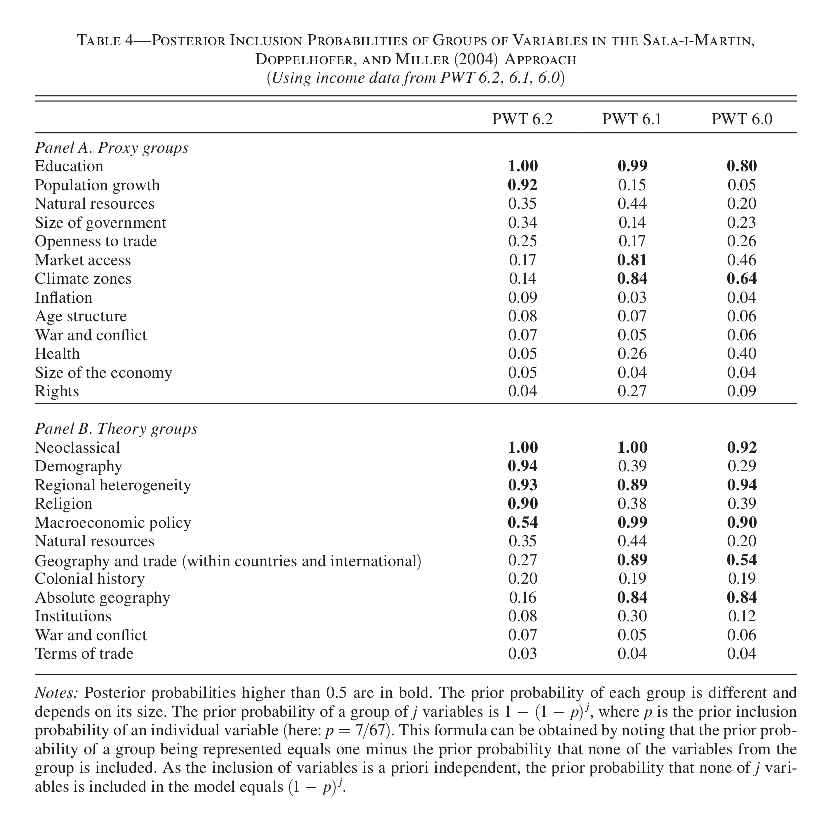
\includegraphics[scale=.5]{ciccone.eps}
  \end{figure}
\end{frame}
%--------------------------------------


%--------------------------------------
\begin{frame}
  Growth accounting studies rely on estimate of GDP, however GDP is often badly measured
  \begin{itemize}
    \item Need to measure nominal GDP as well as reliable price indices
  \end{itemize}
  \medskip
  Particularly a problem in developing countries due to number of factors
  \begin{enumerate}
    \item Smaller fraction of economic activity is formal
    \item Economic integration within-country is lower
    \item Statistical infrastructure is weak
  \end{enumerate}
\end{frame}
%--------------------------------------

%--------------------------------------
\begin{frame}
  Henderson et al. (2012) provide a solution using night-light emissions measured by satellites
  \begin{itemize}
    \item Lights at night are conspicuous consumptions
    \item Can serve as proxy for economic activity; both short and long term
  \end{itemize}
\end{frame}
%--------------------------------------

%--------------------------------------
\begin{frame}
  \begin{figure}
    \includegraphics[scale=.12]{noaa.eps}
  \end{figure}
\end{frame}
%--------------------------------------

%--------------------------------------
\begin{frame}
  Henderson et al. (2012) use the following framework to relate lights to GDP growth.\\
  First, there is classical measurement error in GDP data
  \begin{align}
    z_j= y_j+\epsilon_{z,j}
  \end{align}
  $z$ the growth of real GDP as measured in national income accounts\\
  $y$ is growth in true real GDP\\
  $j$ indexes country, $\epsilon_z$ is denoted $\sigma^2_z$
\end{frame}
%--------------------------------------

%--------------------------------------
\begin{frame}
  Second, relation between growth of lights and true income is given by
  \begin{align}
    x_j=\beta y_j + \epsilon_{x,j}
  \end{align}
  \medskip
  i.e. there is a simple constant elasticity between total observable lights $X$ and total income $Y$
  \begin{align}
    X_j=Y_j^{\beta}
  \end{align}
  \medskip
  For predictive purpose we are interested in
  \begin{align}
    z_j=\hat{\psi} x_j + e_j
  \end{align}
\end{frame}
%--------------------------------------

%--------------------------------------
\begin{frame}
 OLS parameter $\hat{\psi}$ is simply $cov(x,z)/ cov(x)$; relationship between $\hat{\psi}$ and structural parameter $\beta$ is
 \begin{align}
   \hat{\psi} = \frac{1}{\beta} \left( \frac{\beta^2 \sigma^2_y}{\beta^2 \sigma^2_y + \sigma^2_x}     \right)
 \end{align}
 \medskip
 $\hat{\psi}$ is an estimate of the inverse of elasticity of lights with respect to income, but it is a biased estimate
 \begin{itemize}
   \item Due to inversion of production relationship and measurement error in $x$
 \end{itemize}
 Eq. 59 can be used as proxy for best-fit relationship
 \begin{align}
   \hat{z}_j=\hat{\psi}x_j
 \end{align}  
\end{frame}
%--------------------------------------

%--------------------------------------
\begin{frame}
  $\hat{z}$ is a separate estimate of income growth which can be combine with a national account measure to create a composite measure $\hat{y}$
  \begin{align}
    \hat{y}_j=\lambda z_j + (1-\lambda)\hat{z}_j
  \end{align}
  The variance of the composite estimate is given by  
  \begin{align}
    var(\hat{y}-y)=\lambda^2\sigma^2_z + (1-\lambda)^2 \frac{\sigma^2_y \sigma^2_x}{\beta^2 \sigma^2_y + \sigma^2_x}
  \end{align}
  This is solved for the weight $\lambda^*$ which minimises the variance
  \begin{align}
    \lambda^* = \frac{\sigma^2_x \sigma^2_y}{\sigma^2_z(\beta^2 \sigma^2_y + \sigma^2_x) + \sigma^2_x \sigma^2_y}
  \end{align} 
\end{frame}
%--------------------------------------

%--------------------------------------
\begin{frame}
  $\lambda^*$ is a function of four unknown parameters but there are only three known sample moments
  \begin{align}
    var(z) &= \sigma^2_y + \sigma^2_z\\
    var(x) &= \beta^2 \sigma^2_y + \sigma^2_x\\
    cov(x,z) &= \beta \sigma^2_y
  \end{align}
  i.e. for the last moment $cov(y,x)=cov(x,z)$ one more equation is needed, which is based on the assumption about the signal-to-noise ratio in measured GDP growth $z$
  \begin{align}
    \phi= \frac{\sigma^2_y}{\sigma^2_y \sigma^2_z}
  \end{align}
  \medskip
  Assuming a specific value for $\phi$, optimal $\lambda$ will be given by
  \begin{align}
    \lambda^* &= \frac{\phi var(z)var(x) -cov(z,x)^2}{var(z)var(x)-cov(z,x)^2} \\ \nonumber
     &= \frac{\phi-\rho^2}{1-\rho^2}
  \end{align}
  with $\rho$ being the correlation between $z$ and $x$
\end{frame}
%--------------------------------------

%--------------------------------------
\begin{frame}
  \begin{figure}
    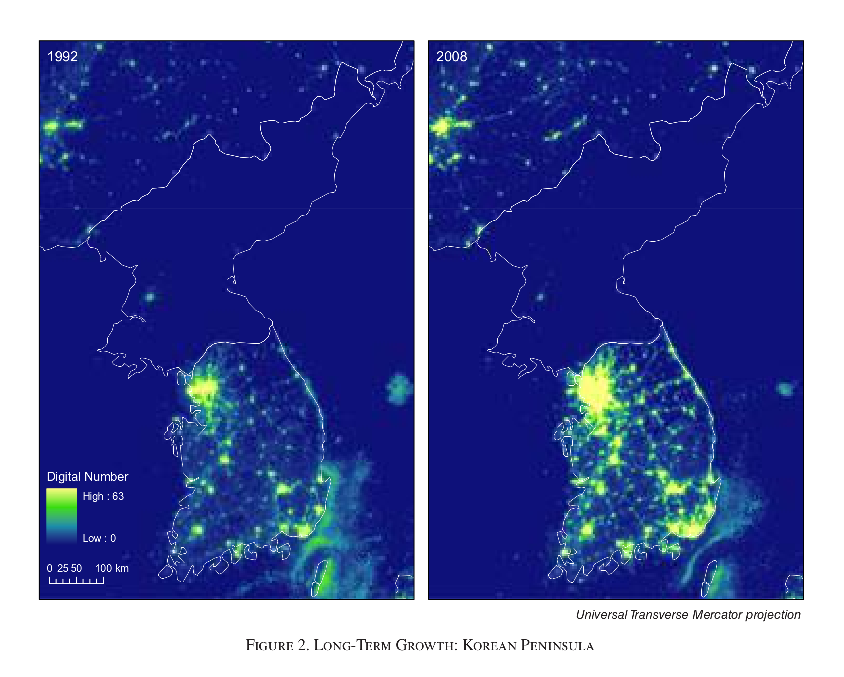
\includegraphics[scale=.7]{henderson_et_al.eps}
  \end{figure}
\end{frame}
%--------------------------------------

%--------------------------------------
\begin{frame}
  \begin{figure}
    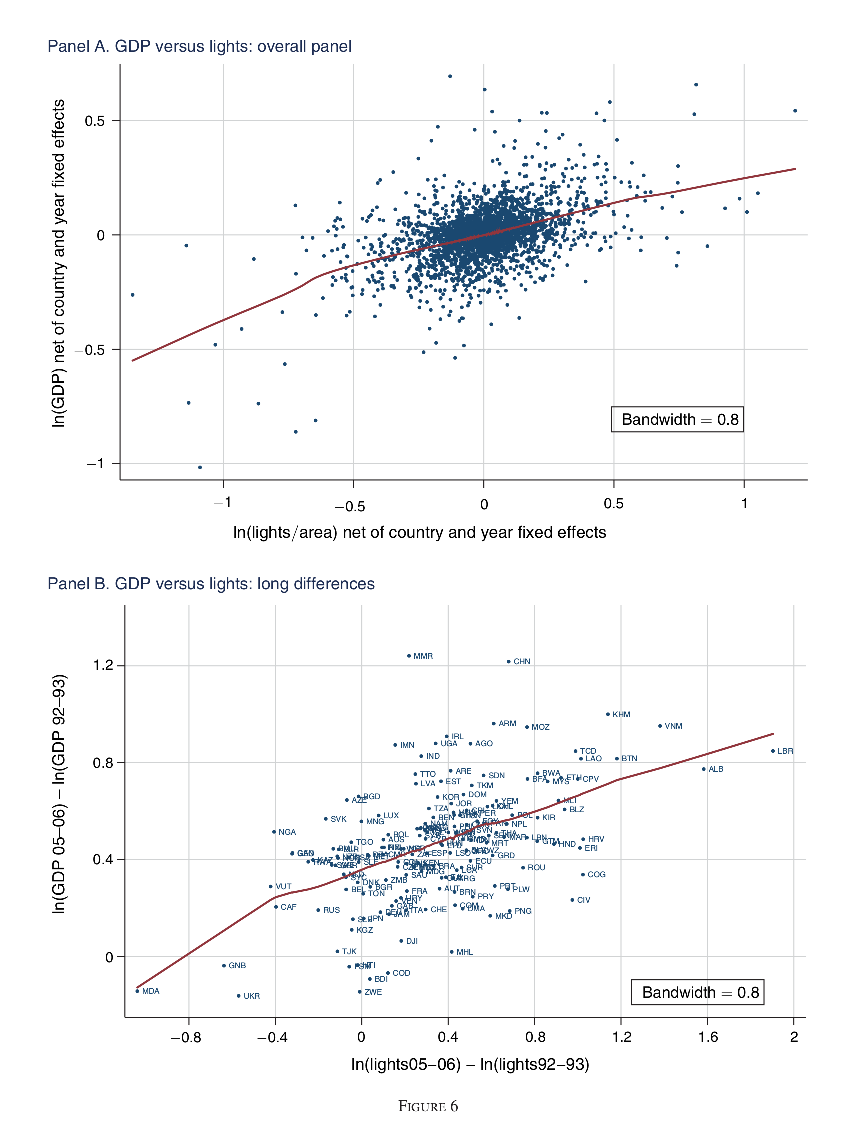
\includegraphics[scale=.45]{henderson_et_al2.eps}
  \end{figure}
\end{frame}
%--------------------------------------

%--------------------------------------
\begin{frame}
  \begin{figure}
    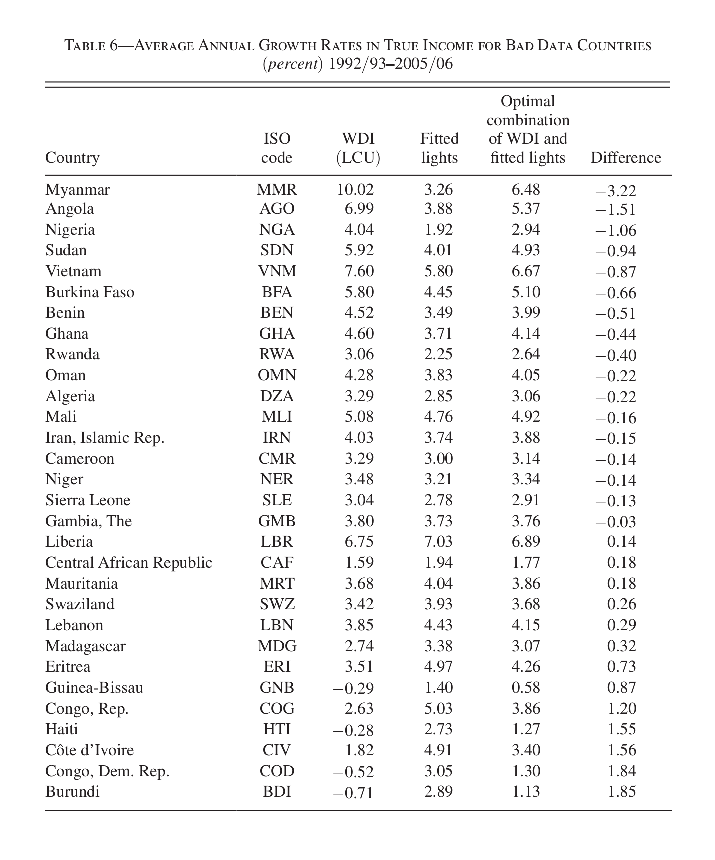
\includegraphics[scale=.45]{henderson_et_al3.eps}
  \end{figure}
\end{frame}
%--------------------------------------


%--------------------------------------
\end{document}
